\documentclass[journal]{IEEEtran}

% *** CITATION PACKAGES ***
%
\ifCLASSOPTIONcompsoc
  \usepackage[nocompress]{cite}
\else
  % normal IEEE
  \usepackage{cite}
\fi
% *** GRAPHICS RELATED PACKAGES ***
\ifCLASSINFOpdf
	\usepackage[pdftex]{graphicx}
\else
	\usepackage[dvips]{graphicx}
\fi
\usepackage{amsmath}
%
%\usepackage{algorithmic}
%\usepackage{algorithm}

%\usepackage{algorithmicx}

\usepackage[linesnumbered,ruled,vlined]{algorithm2e}

%\usepackage[noend]{algpseudocode}
\usepackage{array}
\ifCLASSOPTIONcompsoc
  \usepackage[caption=false,font=footnotesize,labelfont=sf,textfont=sf]{subfig}
\else
  \usepackage[caption=false,font=footnotesize]{subfig}
\fi
\usepackage{fixltx2e}
% \usepackage{stfloats}
\usepackage{tikz}
\usepackage{dblfloatfix}
\usepackage{url}
\usepackage{comment}
\usepackage{color}
\usepackage{subfloat}
\usepackage[automake, acronym]{glossaries}
\usepackage{widetext}
%\usepackage{subcaption}
%\usepackage{subfigure}
\usepackage[keeplastbox]{flushend}
\newtheorem{theorem}{Theorem}[section]

%configure hyphenation
\lefthyphenmin8
\righthyphenmin8
\hyphenation{op-tical net-works semi-conduc-tor}

\loadglsentries{tex/abbrs.tex}
\makeglossaries


\newcommand{\notesc}[1]{\textcolor{red}{SC: #1}}
\newcommand{\noteam}[1]{\textcolor{green}{Abhijit: #1}}
\newcommand{\notesb}[1]{\textcolor{blue}{Sourav: #1}}



\let\oldnl\nl% Store \nl in \oldnl
\newcommand\nonl{%
	\renewcommand{\nl}{\let\nl\oldnl}}

\begin{document}
%\title{MPIoT: A simpler transport protocol}
\title{Viscous: An End to End Protocol for Ubiquitous Communication over Internet of Everything}

\author{\IEEEauthorblockN{Abhijit Mondal, Sandip Chakraborty\\}
\IEEEauthorblockA{Department of Computer Science \& Engineering\\
	Indian Institute of Technology, Kharagpur\\
	Kharagpur, India 731303\\
	Email: abhimondal@iitkgp.ac.in, sandipc@cse.iitkgp.ernet.in}
}

% conference papers do not typically use \thanks and this command
% is locked out in conference mode. If really needed, such as for
% the acknowledgement of grants, issue a \IEEEoverridecommandlockouts
% after \documentclass

% for over three affiliations, or if they all won't fit within the width
% of the page (and note that there is less available width in this regard for
% compsoc conferences compared to traditional conferences), use this
% alternative format:
% 
%\author{\IEEEauthorblockN{Michael Shell\IEEEauthorrefmark{1},
%Homer Simpson\IEEEauthorrefmark{2},
%James Kirk\IEEEauthorrefmark{3}, 
%Montgomery Scott\IEEEauthorrefmark{3} and
%Eldon Tyrell\IEEEauthorrefmark{4}}
%\IEEEauthorblockA{\IEEEauthorrefmark{1}School of Electrical and Computer Engineering\\
%Georgia Institute of Technology,
%Atlanta, Georgia 30332--0250\\ Email: see http://www.michaelshell.org/contact.html}
%\IEEEauthorblockA{\IEEEauthorrefmark{2}Twentieth Century Fox, Springfield, USA\\
%Email: homer@thesimpsons.com}
%\IEEEauthorblockA{\IEEEauthorrefmark{3}Starfleet Academy, San Francisco, California 96678-2391\\
%Telephone: (800) 555--1212, Fax: (888) 555--1212}
%\IEEEauthorblockA{\IEEEauthorrefmark{4}Tyrell Inc., 123 Replicant Street, Los Angeles, California 90210--4321}}




% use for special paper notices
%\IEEEspecialpapernotice{(Invited Paper)}




% make the title area
\maketitle



\begin{abstract}

Adaptive bitrate video streaming over the Internet typically uses HTTP over TCP. Lately Quick UDP Internet Connection (QUIC) protocol, introduced by Google, has been shown to improve web browsing performance over TCP. Engineered to have better connection establishment, congestion control, and stream multiplexing capabilities, QUIC seems to be an obvious candidate for replacing TCP for video streaming over the web. In this work, we focus on comparing adaptive bitrate streaming performance over QUIC and TCP. Our experimental analysis is based on $175$ YouTube video streams that are accessed from a browser, and over a controlled network setup such that impact of different parameters can be studied. We observe that QUIC is better in maintaining a higher bitrate during playback, as well as, reduces bitrate switching, relative to TCP. However, QUIC uses more bandwidth to download higher data volume for buffering, especially at low bandwidth, and even suffers from more rebuffering events during playback compared to the use of TCP.

%Quick UDP Internet Connection (QUIC) is an experimental protocol developed by Google, which claims to solve the connection setup and congestion control overhead of popular Transmission Control Protocol (TCP) for large number of parallel data flows over the Internet, while providing an end-to-end secure connection. 
%The existing studies of QUIC performance show that it is good for web access as it is a light-weight protocol and can significantly reduce page download time compared to TCP. 
%However, a large number of todays' Internet traffic is based on multimedia streaming applications, such as NetFlix, YouTube and so on, and it is not known whether or how QUIC can improve the adaptive streaming performance over the web, compared to TCP. 
%In this work, we have downloaded around $175$ video clips of different types (video length, content encoding, content type) under controlled and monitored network conditions using both QUIC and TCP, and analyzed the adaptive streaming performance for both the scenarios. 
%We have observed that QUIC aggressively download high quality video segments even at low bandwidth, however it suffers from large number of re-buffering compared to TCP. 
%Further, due to quality switching during adaptive streaming, QUIC also wastes a large amount of data compared to TCP.

\end{abstract}

% no keywords




% For peer review papers, you can put extra information on the cover
% page as needed:
% \ifCLASSOPTIONpeerreview
% \begin{center} \bfseries EDICS Category: 3-BBND \end{center}
% \fi
%
% For peerreview papers, this IEEEtran command inserts a page break and
% creates the second title. It will be ignored for other modes.
\IEEEpeerreviewmaketitle

%\section{Introduction}
%During the last decade, social video streaming for targeted audiences have seen a huge boom with applications like Twitch.tv, Periscope, Meerkat along with the traditional YouTube \& Facebook live and similar other personalized live streaming services~\cite{wang2016anatomy}. Live broadcasts over such platforms have increased many-folds during the recent COVID-19 pandemic due to over-the-top (OTT) services like online live broadcast of classroom lectures to the students\footnote{\url{https://www.nokia.com/blog/network-traffic-insights-time-covid-19-march-23-29-update/} (Accessed: \today)}. Many existing studies indicate that live streaming of popular events, such as a live cricket or football match, creates multiple traffic bottlenecks in the network, particularly at the Internet gateways of private organizational networks or Internet Service Providers (ISP)~\cite{yan2018understanding}. Consequently, a question arises -- how can we prevent traffic bottlenecks in the Internet while allowing high definition video streaming to millions of users? 

In the previous chapters, we have analyzed the online video streaming systems and developed a way to reduce the energy consumption while streaming online videos. In this chapter, we consider a class of live but non-interactive streaming applications, where the video is broadcast to a set of targeted audiences over social streaming applications. Social streaming applications many-a-times form communities which are localized, forming one or more geographical clusters~\cite{wang2016anatomy}. We utilize this localized community formations among live streaming viewers to construct one or more playback coalitions, as shown in \fig\ref{fig:chap06:flsd}. The coalition members share a common network gateway (such as an organizational local network gateway or the service gateway for a cellular core network) to connect to the Internet, however, there are direct high-speed local connections among the coalition members (like \acr{LAN} connections or cellular device-to-device connections). It can be noted that such a coalition can be formed based on the principles of \ac{ALTO}, where an \ac{ALTO} server can provide the locality information of video players without requiring any explicit network or device firmware change. The coalition members collectively download the video from the content provider based on an \ac{ABR} streaming strategy, such as \ac{DASH}. The clients in a coalition collectively decide the adaptive playback rate and share data-download loads among themselves maintaining the playback synchronization. 
\begin{figure}[!ht]
    \centering
    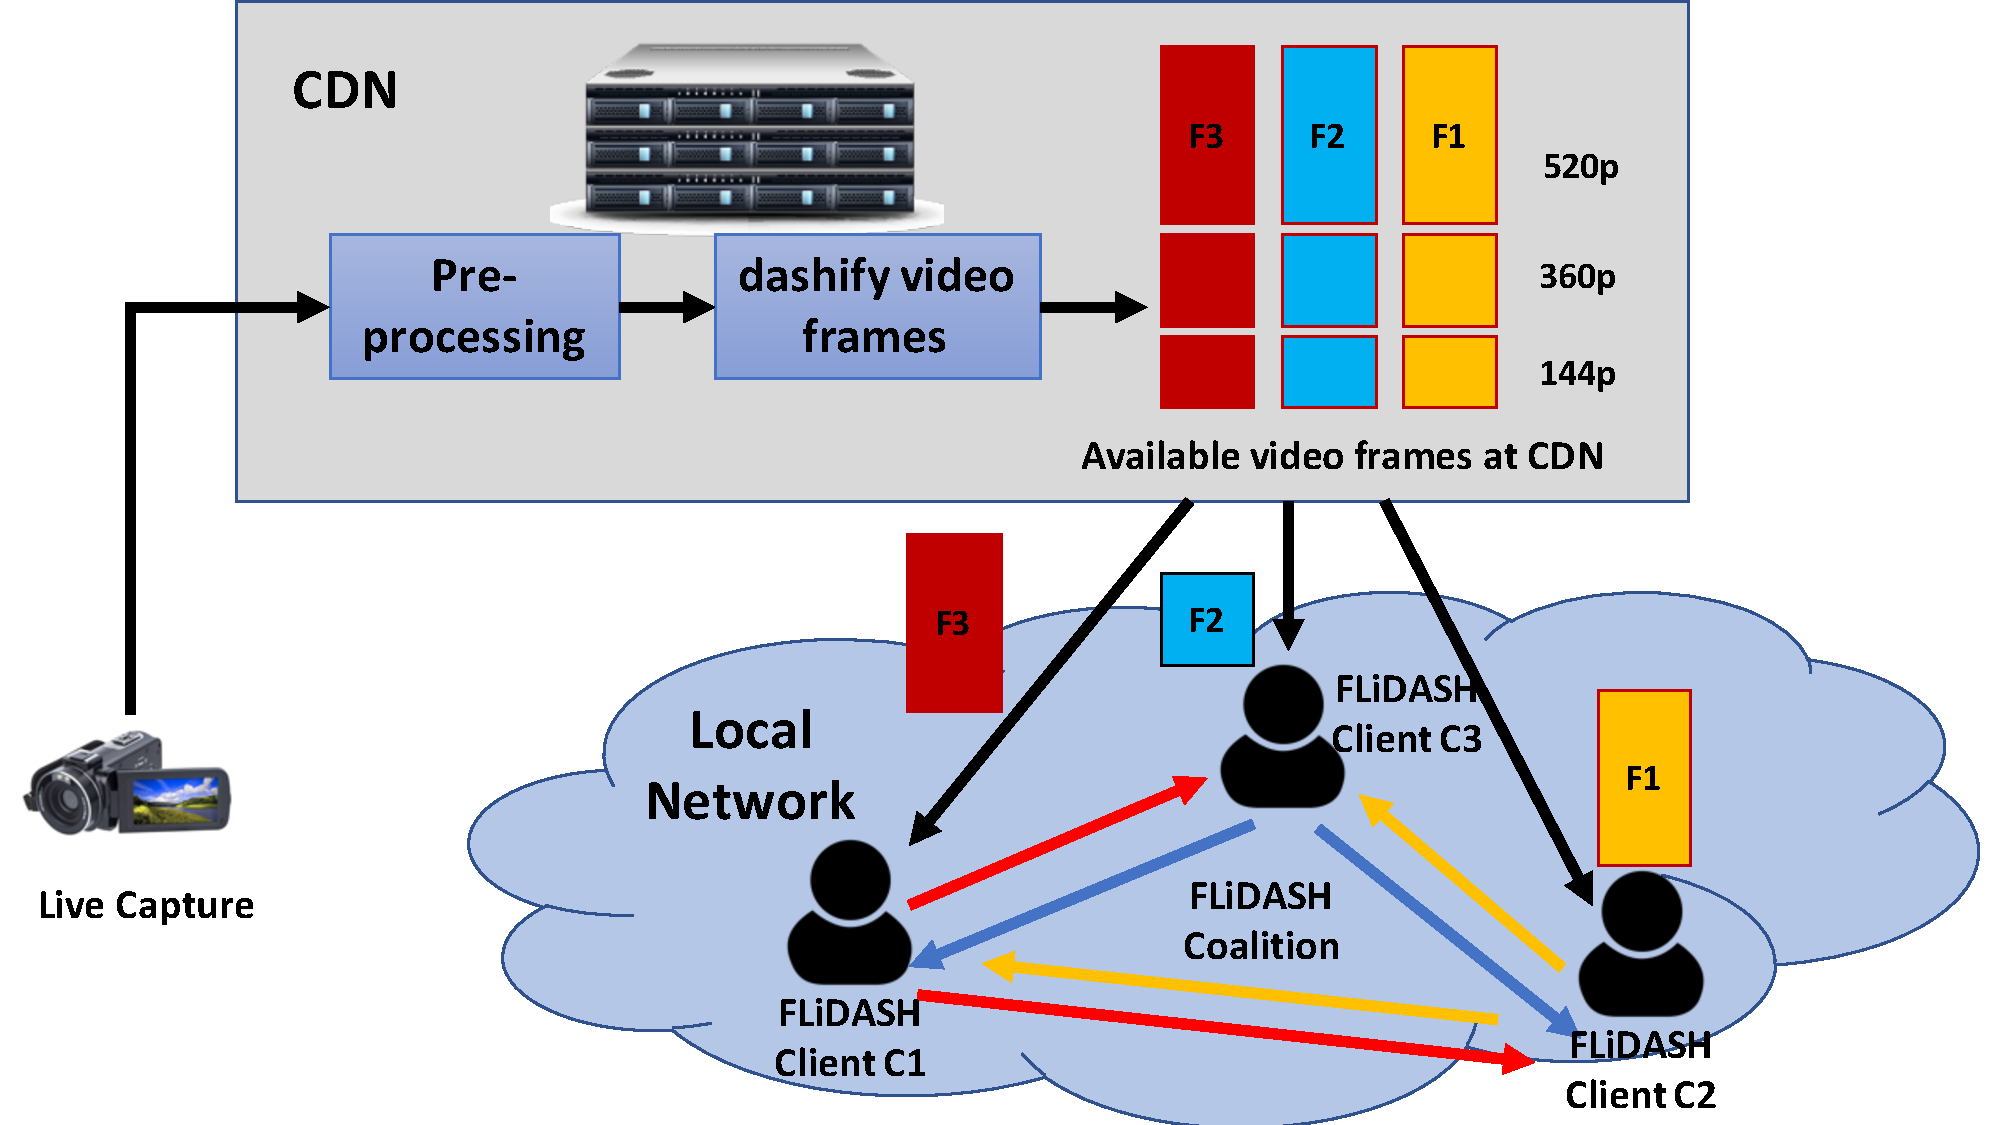
\includegraphics[width=0.8\linewidth]{img/flsd.pdf}
    \caption{Overview of \our: The clients under a local network create a coalition, every members of the coalition share the total download load.}
    \label{fig:chap06:flsd}
\end{figure}

However, developing such a system has multiple challenges. First, the coalition needs to be designed in a way such that downloading data directly from the content provider is costlier than sharing the data over the local network. Second, there should be a proper distribution of segment-wise data-download scheduling among the coalition members such that playback synchronization is not violated. A proper playback synchronization ensures that every player in the coalition should acquire the video segment $s_{i}$, either downloaded by itself or fetched from another coalition player through the direct local link, by the time it completes playing the previous video segment $s_{i-1}$; otherwise, there might be a rebuffering delay affecting the \ac{QoE}. Third, the Internet bandwidth of individual players may vary over time; therefore, the coalition as a whole should schedule the video segment downloads among its members as well as decide the bitrate of every video segment based on the \ac{ABR} principle.

Owing to the above challenges, we develop a coalition-based adaptive live streaming  called \textit{Federated Live Streaming over \ac{DASH}} (\our) where the streaming clients or players form a dynamic coalition based on the network quality parameters and collectively stream a live video. We use the playback buffer statistics at individual streaming clients to develop a distributed mechanism for coalition formation with the help from a proximity server (which can be an \ac{ALTO} server). The members of a coalition use a low-overhead gossip-based protocol for playback synchronization and takes following two decisions -- (1) scheduling the downloads of video segments among the coalition members based on their individual instantaneous network condition and the overall fairness criteria, and (2) bitrate of each video segments to optimize the overall \ac{QoE} of the coalition. We use the following \ac{QoE} objectives while making the above decisions -- (a) improve the overall video quality level, (b) improve the playback smoothness by reducing the quality fluctuations, (c) reduce rebuffering, and (d) improve fairness  among the coalition members in terms of the downloaded data share. We have implemented {\our} over an emulated environment and have thoroughly compared its performance with various other baselines. We observe that {\our} improves the overall \ac{QoE} with less traffic overhead at the backbone network.

The rest of the chapter is organized as follows. 


\section{Related works and their limitations} 
A number of recent research works, such as~\cite{yadav2016msocket,abdrabou2016experimental,de2016observing,de2016throughput,islam2016start,maity2017tcp,liu2016improving,mpquic-measure} and the references therein, have revisited the TCP design fundamentals considering the needs for optimization at the transport layer, so that the available network capacity can be fully utilized for both the event driven short-lived traffic as well as the real time multimedia streaming traffic.
Consequently, the network community has explored end-to-end protocols to support the above mentioned features at the transport layer. 
{\em Multi-path TCP}~\cite{paasch2014multipath} has been developed for this purpose, where the connection between a sender and a receiver is established via multiple paths through multiple interfaces. A large number of recent works, such as~\cite{oh2016feedback,barik2016lisa} and the references therein, have explored various aspects of MPTCP and measured its performance over dynamic Internet traffic scenarios. However, as explored in~\cite{kheirkhah2016mmptcp}, MPTCP does not perform well for short flows. 
To address the issue of short-lived flows, Dukkipati \textit{et. al.}~\cite{largecwnd} have suggested to use an initial congestion window size of at least $10$, so that the flows can come out of the slow start phase. 
Later Google has developed an application layer protocol called SPDY~\cite{erman2015towards}, that can multiplex multiple web requests over a single TCP connection. However, it suffers from the {\em Head of Line} (HOL) blocking issue; where if one or more packets get lost during transmission, all the flows need to wait until TCP recovers the lost packets. To address the HOL blocking issue, Google has further developed a UDP based experimental protocol called QUIC~\cite{carlucci2015http,cui2017innovating}. QUIC is similar to SPDY, but it uses UDP as the transport layer protocol instead of TCP. QUIC can handle reliability, congestion control and flows control over the Internet. QUIC is developed on top of connection less UDP protocol. Which is a problem for user behind a NAT. So, QUIC developed in such a way so that it can survive port change in the client. However it can not change IP address \cite{quic-deployment}. Also, being an application layer protocol, it does not have any control over the path it selects; and the path selection mechanism is completely dependent on the underlying routing algorithm. Therefore, QUIC is not a truly multi-path protocol and does not support multihoming and mobility. To address these issue, Coninck {\em et. al.} developed MPQUIC in \cite{mpquic-measure} to add support for multi-path and mobility. However, it still have dependency of network stack and it can not decide interface to send the a segment/packet. So, it may not be able to utilize all the interfaces available in a device. 


\section{Motivation Behind the Research Work}

MPTCP is the most widely explored alternative for TCP, which supports multiple paths through multiple interfaces, while providing TCP like congestion control and reliability features for end-to-end connection. As mentioned earlier, a large number of researches~\cite{oh2016feedback,barik2016lisa,khalili2013mptcp,kheirkhah2016mmptcp,kheirkhah2015short} have explored MPTCP as an alternative of TCP for various application and network scenarios. However, MPTCP has two major shortcomings that prevent its large scale deployment over the Internet -- (a) MPTCP is implemented as a part of the Linux kernel, and therefore requires device reconfiguration for its deployment; and (b) MPTCP is still under exploration phase, and there are multiple shortcomings of MPTCP as pointed out by existing researches. In~\cite{khalili2013mptcp}, Khalili \textit{et al.} have claimed that MPTCP is not pareto optimal. Further, in~\cite{kheirkhah2016mmptcp}, the authors have pointed out that MPTCP is not suitable for short connections. 

Here, we first explore whether we can develop a MPTCP like protocol, or augment MPTCP so that we can support better network utilization for short flows. For this, we ask the following question: \textit{Why does MPTCP perform poorly for short flows?}  To get the answer, we do an emulation setup with the help of \texttt{Mininet} environment~\footnote{\url{http://mininet.org/} (last accessed: 24 April 2017)}, where we setup a network with two multi-homed hosts, and two distinct paths between the two hosts. We vary the end-to-end latency for the two paths, and then transfer data between the two hosts. For our experiment, we have configured the Linux kernel of the hosts with MPTCP version 0.91~\footnote{\url{http://multipath-tcp.org/} (last accessed: 24 April 2017)}. For this experiment, we set the path bandwidth as $50$ Mbps for both the paths. Among the two hosts, one host acts as the MPTCP server, while the other works as the MPTCP client. We keep a file at the server, and download that file from the client through MPTCP based connection. To observe the MPTCP behavior for various connection types, we vary the size of the file, and measure the impacts. 
%
%\begin{figure*}[ht]
%	\captionsetup[subfigure]{}
%	\begin{center}
%		\subfloat[\label{fig:percentSentOverPathRTT80}RTT=80ms]{
%			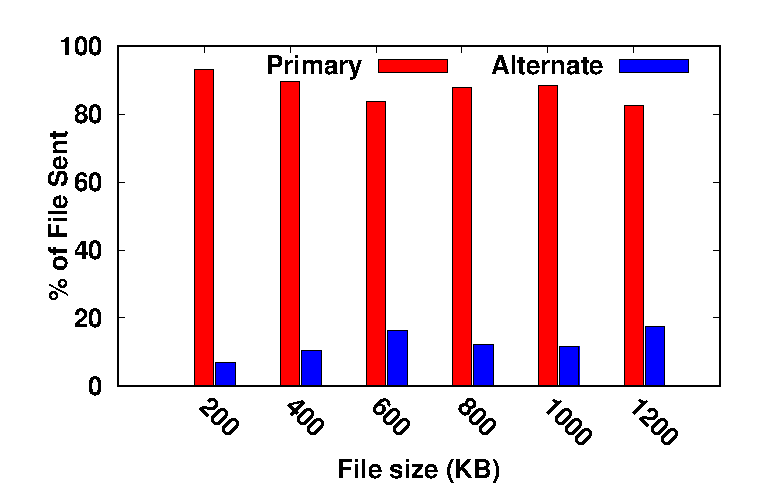
\includegraphics[width=0.32\linewidth]{img/exp4/delay-5}
%		}
%		\subfloat[\label{fig:percentSentOverPathRTT160}RTT=160ms]{
%			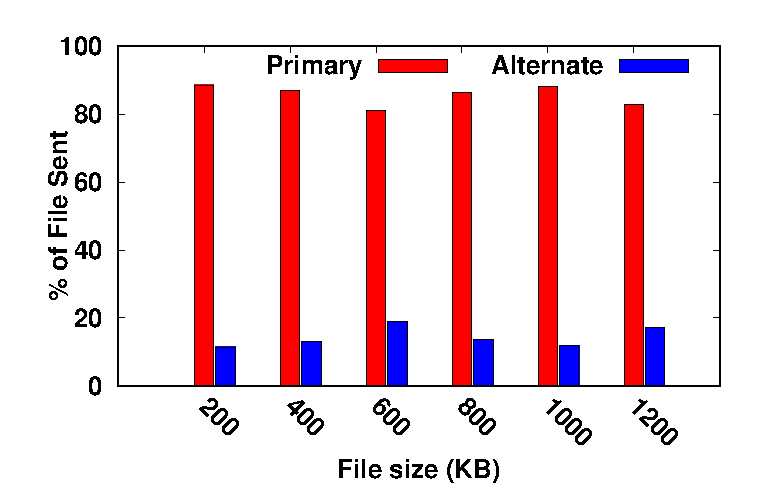
\includegraphics[width=0.32\linewidth]{img/exp4/delay-10}
%		}
%		\subfloat[\label{fig:percentSentOverPathRTT320}RTT=320ms]{
%			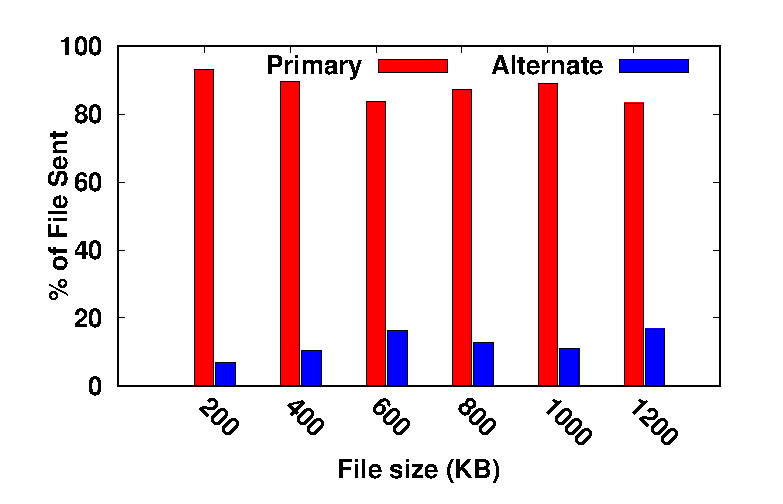
\includegraphics[width=0.32\linewidth]{img/exp4/delay-20}
%		}
%		
%		\caption{\label{fig:percentSentOverPath}\% of data share of a path.}
%	\end{center}
%\end{figure*}

\begin{figure}[!t]
	\begin{center}
	\begin{minipage}{0.45\linewidth}
		\centering
		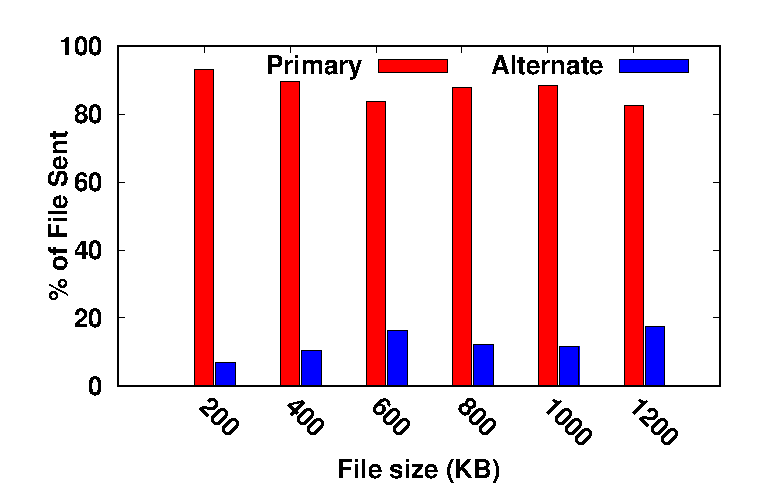
\includegraphics[width=\linewidth]{img/exp4/delay-5}
		\label{fig:percentSentOverPathRTT80}
		\subcaption{RTT=80ms}
	\end{minipage}
	\begin{minipage}{0.45\linewidth}
		\centering
		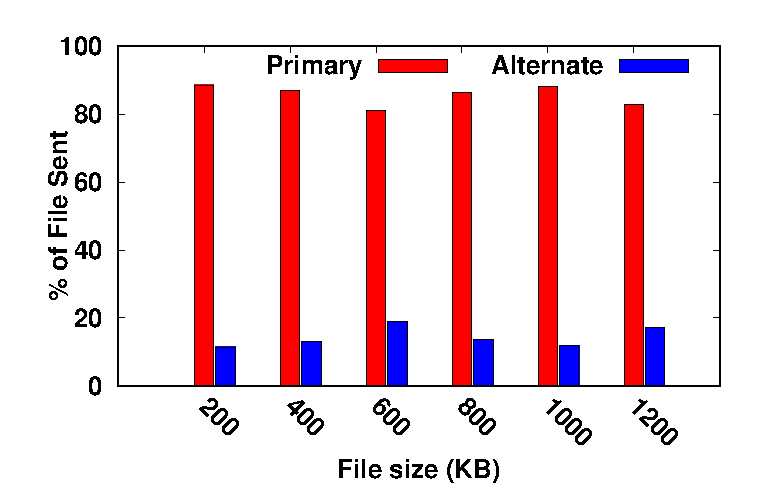
\includegraphics[width=\linewidth]{img/exp4/delay-10}
		\label{fig:percentSentOverPathRTT160}
		\subcaption{RTT=160ms}
	\end{minipage}
	\begin{minipage}{0.45\linewidth}
		\centering
		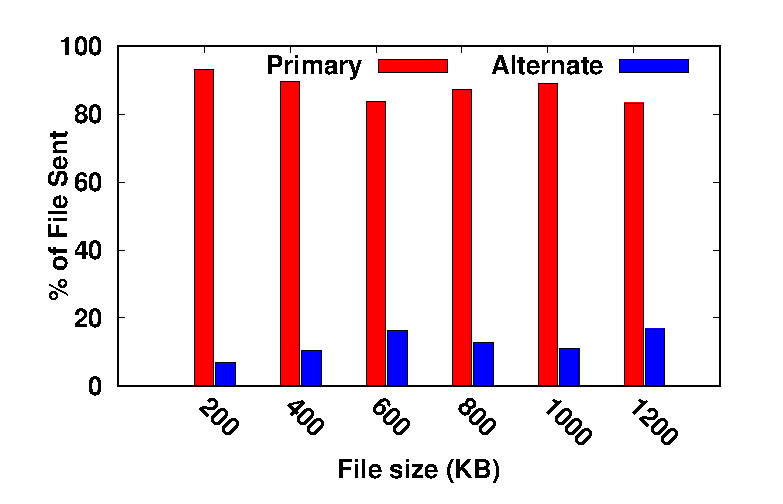
\includegraphics[width=\linewidth]{img/exp4/delay-20}
		\label{fig:percentSentOverPathRTT320}
		\subcaption{RTT=320ms}
	\end{minipage}
	\caption{\label{fig:percentSentOverPath}Percentage of Data Share between the Primary and the Alternate Paths}
	\end{center}
\end{figure}


\subsection{Utilization of Network Bandwidth at Alternate Paths for Short Flows}
MPTCP first initiates the connection through one of the available paths, called the {\em primary path}, and then explores the {\em alternate paths} to initiate alternate connections through them. In the first experiment, we try to look into the amount of data shares between the primary path and the alternate path. For this, we keep the bandwidth and latency for both the paths same, and vary the flow duration by increasing the size of the file to be downloaded at the client from the server. The results are plotted in Fig.~\ref{fig:percentSentOverPath}. We can observe from that figure that there is a huge imbalance between the two paths in terms of data share. The primary path forwards significantly more data compared to the alternate path. By exploring the connection logs, we find that by the time MPTCP sets up a connection to the alternate path, most of the data for a short flow has been transferred over the primary path. Further, the congestion controls for the primary and the alternate paths are handled separately, and therefore the alternate path also needs to go through the slow start phase. Therefore, the alternate path gets severely underutilized for short flows. Further, none of the primary sub-flow (sub-flow over the primary path) and the alternate sub-flow (sub-flow over the alternate path) can reach to the steady state for a short-lived flow.   

%
%We send the different sizes of data over from a host to another host via two separate paths in Mininet, where overall bandwidth and delay in the links are same for both the path. We find out that data share between two paths is imbalanced. We plot the results in Fig.~\ref{fig:percentSentOverPath}. We can see that 80\%-90\% of the data carries by primary path because \acrshort{mptcp} starts secondary sub-flow only after the establishment of the primary connection. By the time, secondary sub-flows establishes connection, primary sub-flow already sent several packets over the network. Primary sub-flow stays at least one \acrshort{rtt} ahead of secondary sub-flow. And none of the flow can reach the steady state for are short-lived flows.
%
%\acrshort{mptcp} can not balance between the different path for short-lived connection.

\subsection{Impact of MPTCP Path Selection During Connection Initiation}
We the perform another experiment on path selection, where the two paths have different round trip time (RTT). Here, we explore the effect of primary path selection, where we ask the following questions -- (a) {\em Does the RTT difference between the primary and the alternate path impact MPTCP performance?}; and (b) {\em Does the MPTCP performance differ if the low RTT path is selected as the primary path?} Consequently, we vary the RTT of the two paths, and the results are plotted in Fig.~\ref{fig:timeSentOverPath}. The two different bars in the graphs show the average file download time for two cases --  (i) low RTT path is used as the primary path, and (ii) high RTT path is used as the primary path. We observe that for small size file download, the performance varies a lot based on the selection of the primary path. However, the primary path selection is not a part of the core MPTCP mechanism, and MPTCP uses the path to set-up the primary sub-flow, which is provided by the underlying routing algorithm.  

%i.e. if \acrshort{mptcp} select longer path as primary path vs. shorter path as the primary path. In this experiment, we find that the time requires to send data using \acrshort{mptcp} over multiple paths largely depends on the primary path selection. For short-lived data and high RTT (Fig.~\ref{fig:timeSentOverPathRTT160}, Fig.~\ref{fig:timeSentOverPathRTT320}), it is taking significantly lesser time if \acrshort{mptcp} select shorter path as primary path. Results are plotted in Fig.~\ref{fig:timeSentOverPath}.
%\notesc{Do not use short and long paths -- use low RTT path and high RTT path in the figure. Use `File Size' instead of `Data Size'; and `Time Required to send Data' to `File Download Time'. }

%\begin{figure*}[ht]
%	\captionsetup[subfigure]{}
%	\begin{center}
%		\subfloat[\label{fig:timeSentOverPathRTT80}RTT: short path=80ms, long path=120ms]{
%			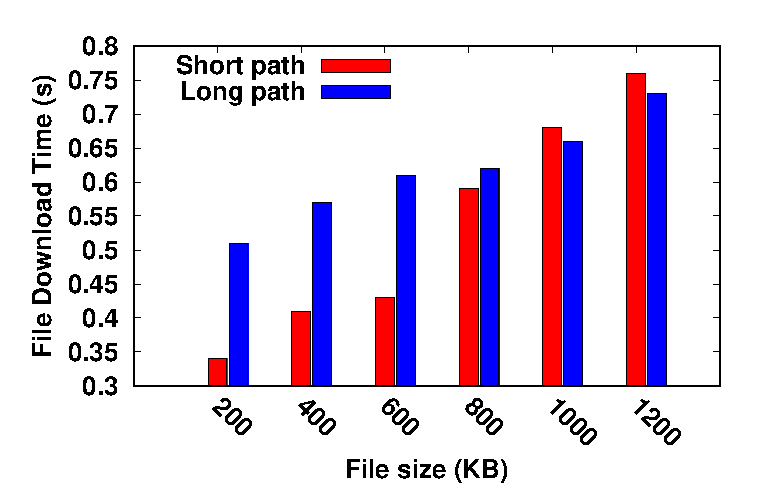
\includegraphics[scale=0.45]{img/exp5/time_needed_5}
%		}
%		\subfloat[\label{fig:timeSentOverPathRTT160}RTT: short path=160ms, long path=240ms]{
%			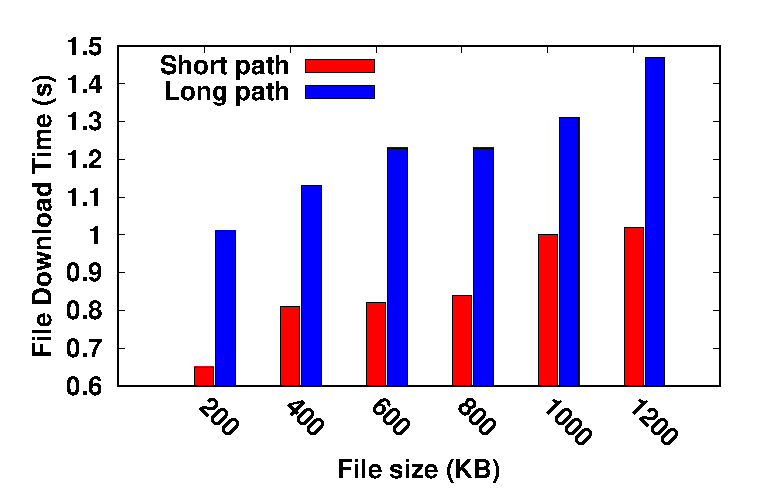
\includegraphics[scale=0.45]{img/exp5/time_needed_10}
%		}
%		\subfloat[\label{fig:timeSentOverPathRTT320}RTT: short path=320ms, long path=480ms]{
%			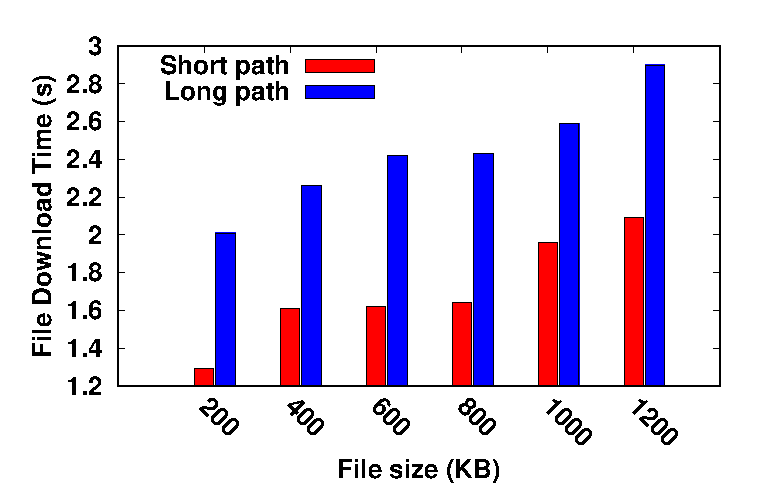
\includegraphics[scale=0.45]{img/exp5/time_needed_20}
%		}
%		
%		\caption{\label{fig:timeSentOverPath}Send data from client to server over 2 path using MPTCP. This is plot of \% of data went through a channel.}
%	\end{center}
%\end{figure*}

\begin{figure}[!t]
	\begin{center}
		\begin{minipage}{0.45\linewidth}
			\centering
			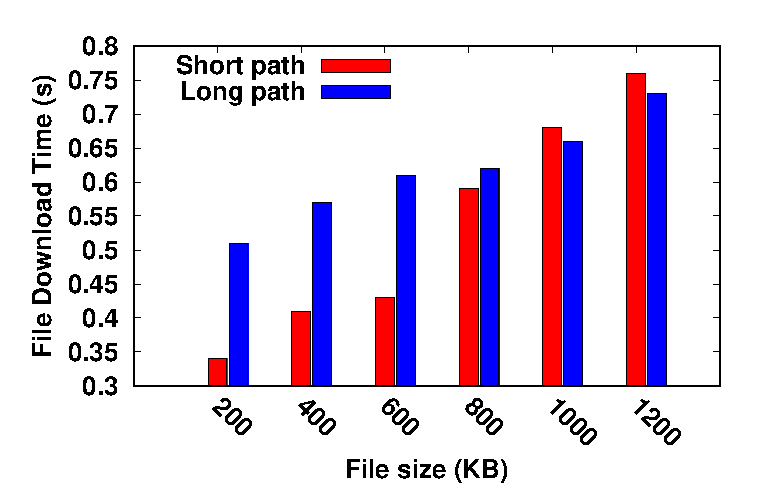
\includegraphics[width=\linewidth]{img/exp5/time_needed_5}
			\label{fig:timeSentOverPathRTT80}
			\subcaption{Short Path RTT: 80ms, Long Path RTT: 120ms}
		\end{minipage}
		\begin{minipage}{0.45\linewidth}
			\centering
			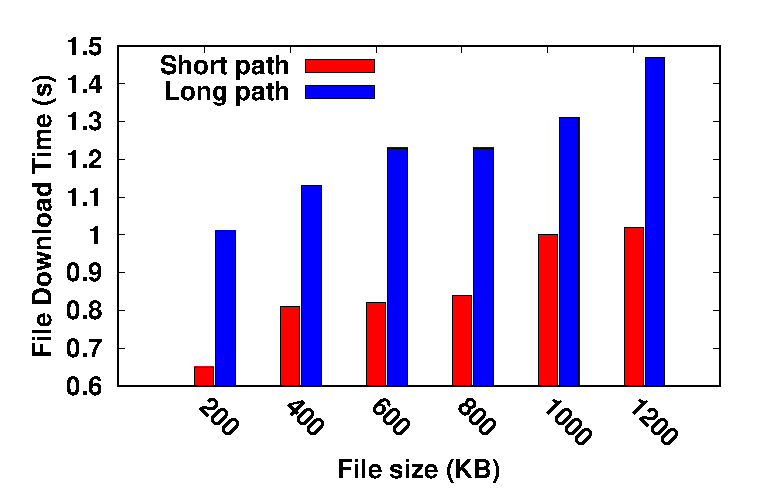
\includegraphics[width=\linewidth]{img/exp5/time_needed_10}
			\label{fig:timeSentOverPathPathRTT160}
			\subcaption{Short Path RTT: 160ms, Long Path RTT: 240ms}
		\end{minipage}
		\begin{minipage}{0.45\linewidth}
			\centering
			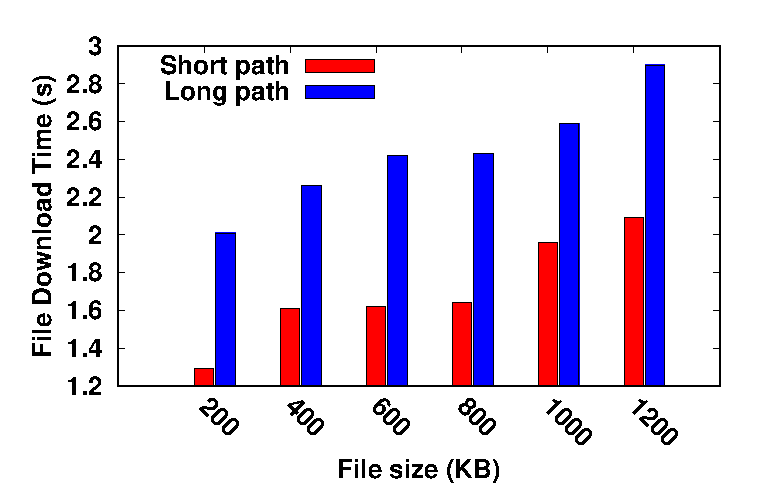
\includegraphics[width=\linewidth]{img/exp5/time_needed_20}
			\label{fig:timeSentOverPathRTT320}
			\subcaption{Short Path RTT: 320ms, Long Path RTT: 480ms}
		\end{minipage}
		\caption{\label{fig:timeSentOverPath}Difference in File Transmission Time based on the Primary Path Selection. The short path indicates the path with the low RTT value, whereas the long path indicates the path with the high RTT value}
	\end{center}
\end{figure}

%\acrshort{mptcp} is incapable of utilizing better path for short-lived connection if it makes mistakes in primary path selection. To overcome these issues and to use multipath, we developed \acrshort{udp} based multi-flow multipath protocol \textbf{Viscous}.
%
%In next section, we describe the protocol and how we overcome the problems with \acrshort{mptcp}.

\subsection{Take Aways}
In summary, the lessons learnt from the above experiments are as follows.
\begin{enumerate}
	\item Connection establishment time is an overhead for short flows. Further flow based congestion control algorithms results in the underutilization of network bandwidth, because every transport layer flow independently increases its transmission rate from the scratch (by increasing the congestion window value for TCP or MPTCP), and the flow may end before its transmission rate reaches to the network capacity. Flow multiplexing at the source device is important to handle such scenarios, however the HOL blocking problem needs to be avoided. 
	\item Connection establishment and path selection cannot be independent for a multi-path protocol, because the performance depends on the path selection mechanism. We need to develop a mechanism where the data transmission can be initiated simultaneously at multiple paths.   
\end{enumerate}
Accordingly, we target to develop a new transport wrapper as a part of this research, that works as a middleware between the application and the transport layer, and provides ubiquitous data transmission between two end hosts while ensuring reliability, flow control and congestion control.  The targeted protocol should use UDP as the transport protocol, and build up the services on top of that. 
%The detailed design philosophy of Viscous along with protocol specifications are discussed in the next section. 

\newpage 

\section{Viscous: Protocol Descriptions}
To overcome the limitations of existing transport layer protocols as discussed in the previous section, we propose a new end-to-end protocol called Viscous. It is a connection oriented multi-path multi-flow protocol which is not coupled with the network stack, and work as a wrapper or a middleware in between the users' application and the transport layer of the network protocol stack. The basic design philosophies for Viscous are as follows. 
\begin{enumerate}
	\item To mitigate the signaling overhead associated with connection establishment, Viscous multiplexes multiple flows over a single Viscous connection. This reduces the connection setup time for short-lived flows. 
	\item Viscous does not maintain a separate and independent congestion control for every application flows. Rather, it maintains a single congestion control mechanism for a Viscous connection which is a multiplex of multiple flows. Further, the congestion control is path specific, that is, congestion is monitored at every path from a source to a destination, where a Viscous sub-flow is initiated.  
	\item To handle HOL blocking problem, Viscous decouples congestion control from the flow control. The Viscous flow control manages the data generation rate from the applications, whereas the congestion control maintains the rate of traffic ingestion into the paths based on congestion feedback. However, to avoid buffer overflow, a feedback is forwarded from the congestion control to the flow control module, whenever necessary.
	\item Viscous follows a modular architecture for ease development of applications. Any Viscous module can be tuned independently to make it suitable for a specific requirement. This way, application layer quality of service (QoS) can be provided with the help of Viscous. 
	\item Viscous works on top of UDP, similar to Goggle's QUIC; therefore it mitigates the transport layer protocol overhead which is associated with TCP. 
	\item Viscous supports different types of mobility without breaking an existing connection. With the help of a unique client and server specific identifier which is shared during the initial connection establishment, Viscous can continue with the existing connection, even if the server or the client changes its IP address.   
\end{enumerate}

\begin{figure}[!t]
	\centering
	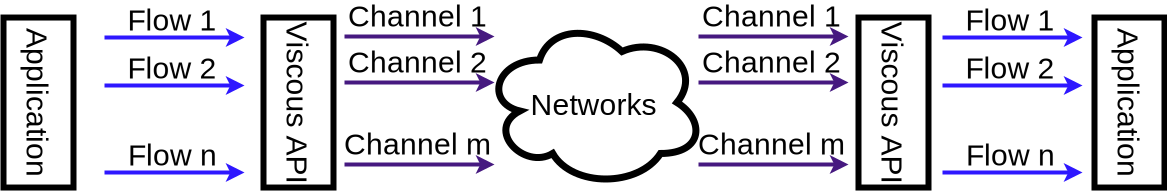
\includegraphics[width=\linewidth]{img/sys-io}
	\caption{Flow-Channel architecture in the Viscous protocol. Application sends and receives data through the flows. Internally, Viscous sends and receives data using multiple channels over multiple paths.}
	\label{fig:sys-io}
\end{figure}

\subsection{Key Concepts Behind the Design of Viscous}
Viscous follows a layered architecture with two different layers, as shown in Fig.~\ref{fig:sys-io}. There are two key concepts behind the design, development, and implementation of Viscous to support ubiquitous transport of data over any Internet devices -- \textit{channel} and \textit{flow}. 

\subsubsection{Channel}
Viscous channels are individual connections between two devices over multiple paths. Paths are defined by compatible source and destination IP pair. There is one single channel for each path. To avoid connection time path imbalance like MPTCP, as we observe in Fig.~\ref{fig:timeSentOverPath}, we initiate all the channels simultaneously after connection establishment and before any flows can start. Connections are established specific to a destination host whenever an application from a source host requests for a connection. This connection is shared with other applications which intend to send data to the same destination host. This way, flows are multiplexed specific to a destination host.

Here connection means Viscous connection. Channels are similar to individual TCP connections or sub-flows in the MPTCP. Each channel has dedicated buffer to provide reliable packet transmission and have congestion control algorithm not to overflow the network. Channels are identified by four tuple of source IP, source interface id, destination IP and destination interface id. Interface id are unique id for each network interface available in a device. All channels are treated as regular, and every channel can participate in transmitting packets from any flows. However, based on other properties like RTT and goodput, one channel can carry more packets than others.


In Viscous, individual application flows do not require separate connection establishment as the connection has already been established between the source and the destination during Viscous connection initiation. Viscous handles congestion control for every individual paths between a source and a destination. Therefore, flow specific congestion control is not required for Viscous, and Viscous maintains path specific congestion control. This way Viscous avoids slow start for every individual flows that share the complete path from the source to the destination. Consequently, channels are persistent in Viscous, and they do not die out after the completion of a flow. As mentioned, a channel can carries data from multiple flows simultaneously by multiplexing them. If one or both the devices are multi-homed, multiple channels can be established that share the traffic load and therefore, achieve better performance.

\subsubsection{Flow} 
Flows in Viscous are responsible for data communication while maintaining the flow-control between a source and a destination. An application can transmit data over multiple flows simultaneously. The user application sends data as byte-streams to the flow, and it also receives data in the form of byte-streams from a flow. Flow is responsible for packetizing the byte-stream and sending the packets to the lower layer of Viscous. Viscous puts packets from flows to channels, and the channels take care of the congestion control. This way, we decouple congestion control from flow control in Viscous design. 

This channel-flow decoupled architecture gives Viscous the power of utilizing multiple paths even for short-lived flows. Flows do not have to suffer from slow start or connection establishment overhead. The connection establishment is a separate event from channel management, and all the channels between a source and a destination start simultaneously. This removes the problem of path selection as we observe in MPTCP.  Further, channel gives an option to support mobility. If one or both the devices change its network address, the associated channel cannot communicate anymore. Viscous can discard the affected channels and initiate new channels using the new network address without any interruption in Viscous connection (application flows). 


\subsubsection{Channel Scheduler}
The Viscous channel scheduler schedules packets from application flows to one of the channels. The channel scheduler have two basic part. i) Load balancer ii) scheduler. The load balancer part is responsible for collecting packets from flows. It is important because it can prioritize one or more flows as per requirement. Although we haven't implemented any priority in our implementation, but we have provision to do it. On the other hand, scheduler is the most important module of our protocol. It decides the way to use multiple channels when different channels have different properties. An ideal scheduler would schedule packet in such a way so that packets arrived on other in ordered fashion. However, to do it, Viscous need to predict future channel condition and application condition which is not feasible. So, we settled with feasible scheduling policies.

First and straightforward way to schedule a packet is to allocate packets to channels in round robin way. In this scheduling policy, scheduler will try to schedule every next packet to next channel if the next channel have space in its $cwnd$, otherwise move next to next channel until scheduler exhaust all the channels. It is easy to deploy, but it is extremely in efficient as we may schedule more packets than required to a slow channel if its $cwnd$ is large.

So, to develop a better scheduler, we developed an acknowledgment(ACK) driven scheduling scheme. Here scheduler schedules a packet to a channel when it receives ACKs and free some space in its $cwnd$. This provides a \textbf{self-clocking behaviour} to the channel scheduler. However, this scheduling works when scheduler buffer always have some packet to send to channels. It is not practical when application trying to send multiple short data. There are phased in between two transmission, when scheduler buffer starves. In those situations, scheduler schedules packets only a channel, and don't put packets to other channels.

Finally, we land to the default MPTCP scheduler. Here, we try to schedule packet packet to a channel with lowest $RTT$ if its $cwnd$ have space for a packet, otherwise move to the channel with second highest $RTT$ and so on. 


\subsection{Connection Establishment: Channels and Flows Creation}

Viscous is a connection oriented protocol. So it uses the client-server architecture for creating and maintaining the connections. A Viscous server waits for a new connection from a Viscous client. 
For each client connection, the server maintains separate sets of channels and other associated modules. In Viscous, communication is possible only after association of the flows to the connections.  

%\begin{figure}[!t]
%	\centering
%	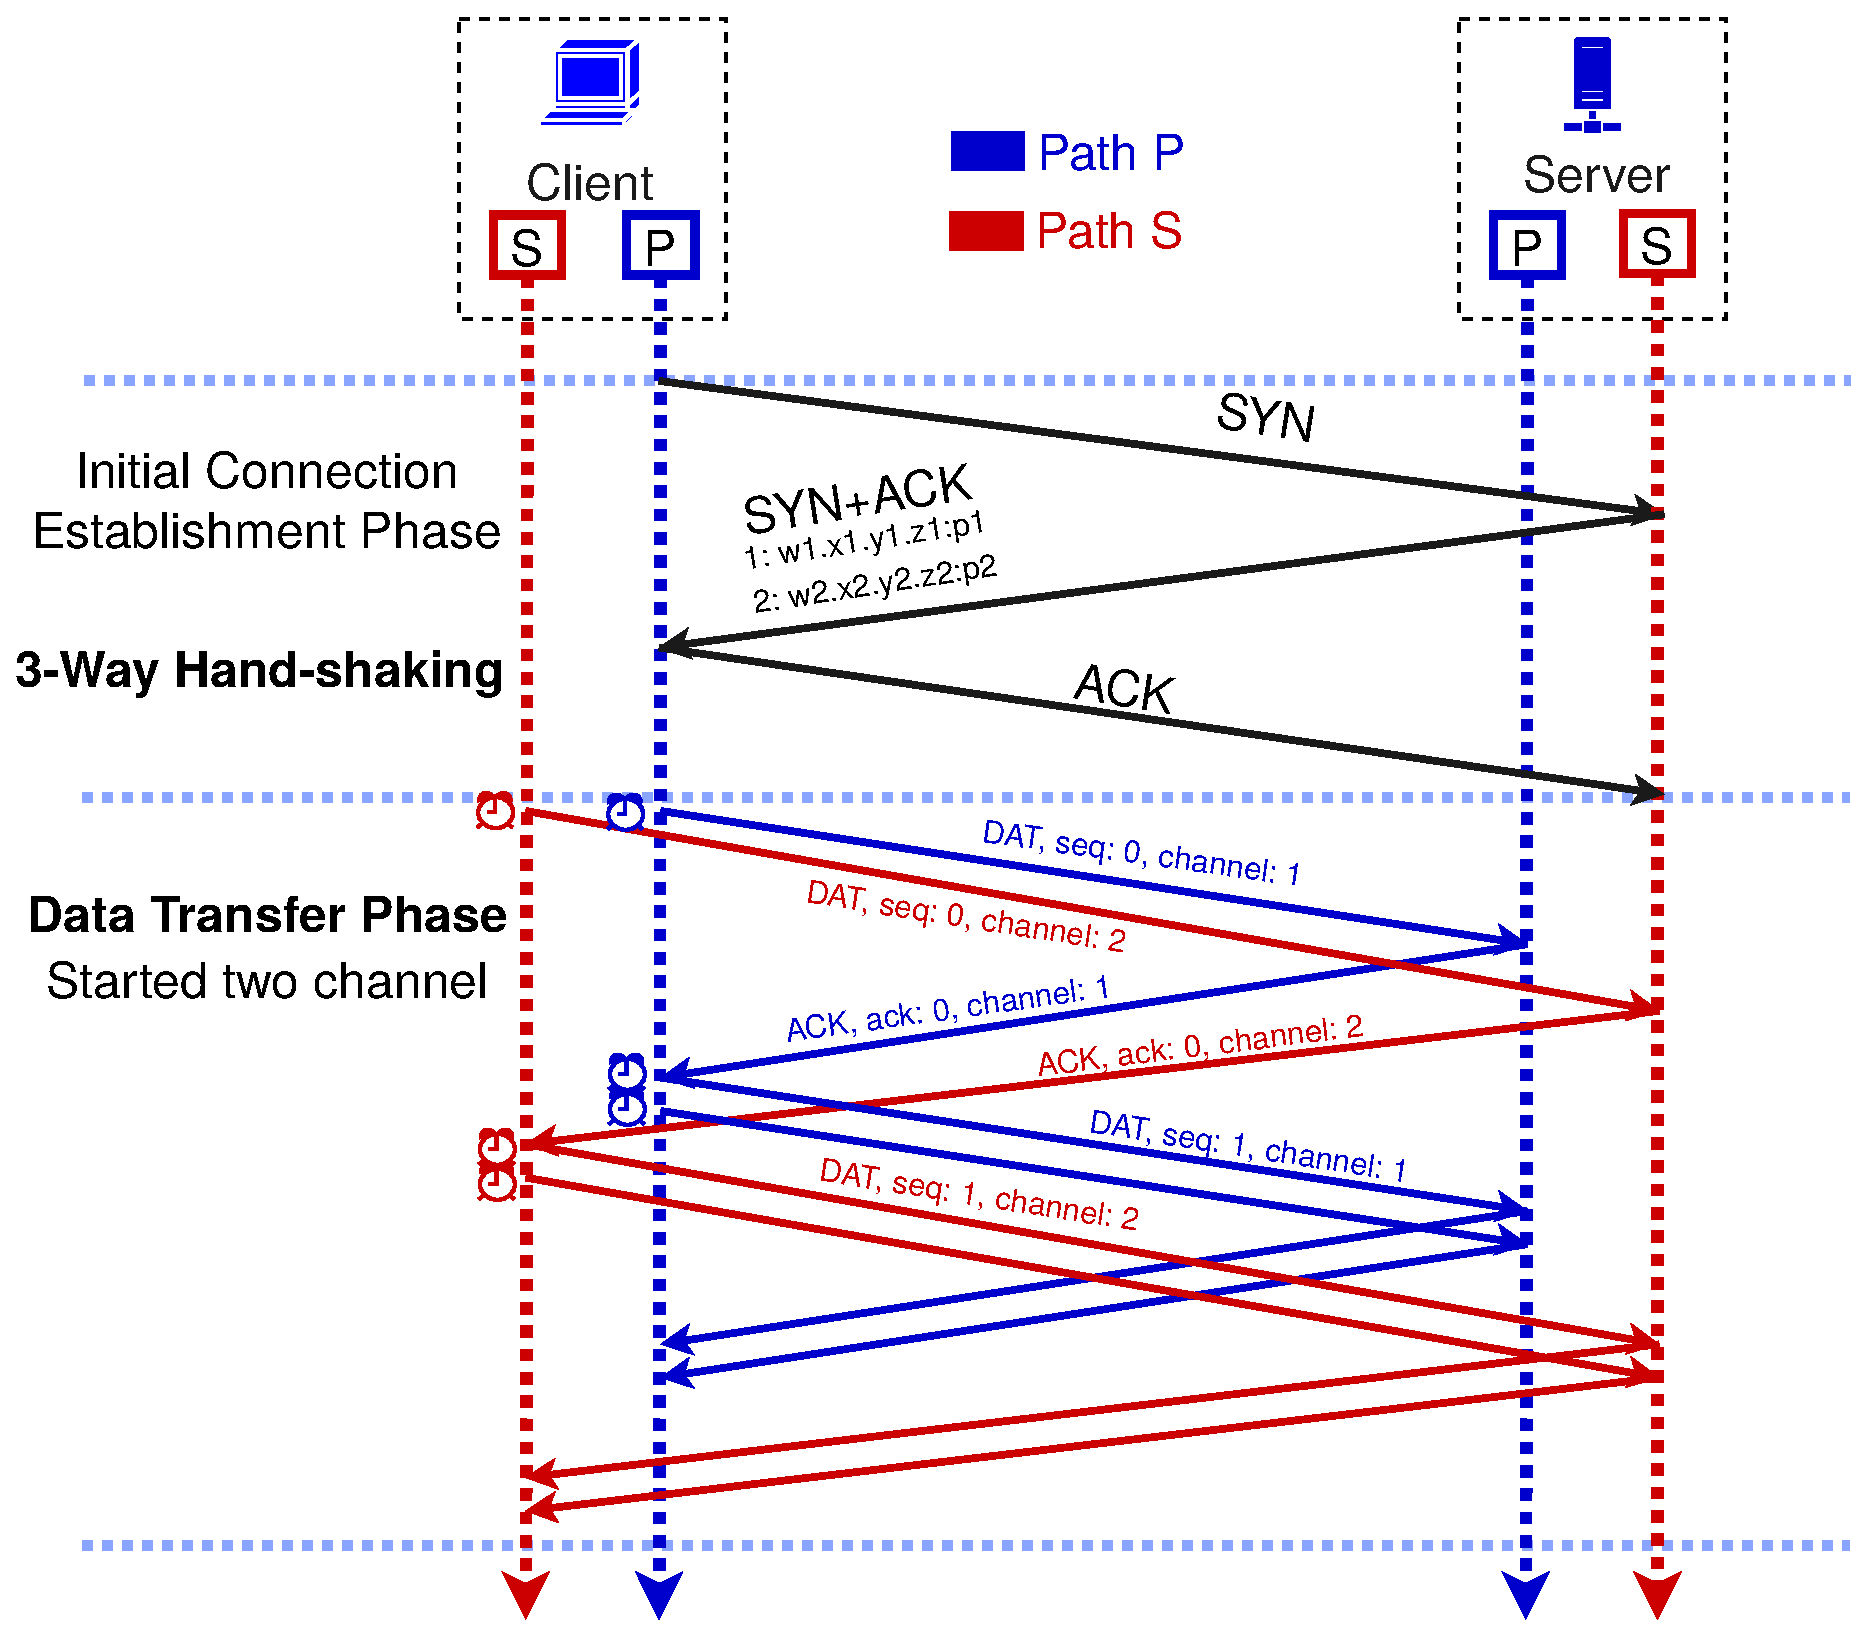
\includegraphics[width=0.8\linewidth]{img/ProtocolDiagram}
%	\caption{Three-way handshaking between client and server and data transfer between them. Handshaking can go between any two pairs of interfaces. Here P is the primary path and S is one of the secondary or alternative paths.}
%	\label{fig:ProtocolDiagram}
%\end{figure}

%Fig.~\ref{fig:ProtocolDiagram} shows the connection establishment and data transmission events for Viscous.
Connection establishment at Viscous follows a three-way handshake procedure similar to the TCP connection establishment. However, as mentioned earlier, Viscous connection establishment is one time and does not depend on the number of flows between the same server, client pair. To establish a connection, a Viscous client sends a synchronization (\texttt{SYN}) packet with a temporary unique identifier or nonce. The nonce or temporary identifier required to identify a client if the \texttt{SYN} packet needs to retransmit. We can use the MAC address of the client as this identifier. On receiving the \texttt{SYN} packet, the Viscous server generates a fingerprint for the client and sends a \texttt{SYN+ACK} packet containing the generated fingerprint. \textit{This fingerprint is used as the connection identifier for the server, client pair}, and every packet between the server and the client includes this fingerprint. In our implementation, we use an SHA256 hash function to generate the fingerprint from the client MAC, server MAC and the current time-stamp used as a unique nonce. It can be noted that different fingerprint is used for different connections, and therefore a fingerprint can uniquely identify a path between a server, client pair. The connection establishment procedure ends with the Viscous client sending an \texttt{ACK} packet. 

During the connection establishment, Viscous server informs all its network addresses to the Viscous client, if the server has multiple interfaces. So, immediately after the connection establishment at one channel, Viscous client initiates all possible channels to Viscous server. There is no requirement to send an extra control packet to complete the channel establishment. After connection establishment, Viscous clients become ready to add flows to the channels, and initiates data transmissions as the applications send data over the flows.

\subsection{Mobility Support in Viscous}
Viscous can support different types of mobility events, as follows.

\subsubsection{Connect-time Mobility}
A connection can fail whenever the server or the client changes its address in between the connection establishment time. With the help of a global name server, this type of mobility can be supported in Viscous. A name server is required to get the new address of the server, when the server changes its IP address. There are two cases that needs to be handled. 
\begin{enumerate}
    \item \textit{Client changes its address just after sending a \texttt{SYN} packet, Server changes its address just after receiving a \texttt{SYN} packet}: This type of failure is automatically recovered by subsequent retries from the client. During the retry, the Viscous client is identified via temporary unique identifier which is used to generate the fingerprint.
    \item \textit{Client or server changes its IP address after receiving the \texttt{SYN+ACK} packet from the server}: As \texttt{SYN+ACK} packet contains the fingerprint, the client can send the \texttt{ACK} packet to complete the three-way handshake by sending the \texttt{ACK} packet to the new server address. The new server address is received with the help from the global name server. However, the success depends on how fast the global name server can update the server IP address against its domain name. If this process fails after three retries, the client re-initiates the connection. 
\end{enumerate}

\subsubsection{Individual Mobility}
Individual mobility event occurs when one of the interfaces from both the devices change its network address. This type of mobility can affect a Viscous connection, only if the affected channel already has some packets under transmission. The subsequent packets will carry the new address to the remote device. This does not create a problem, because the connection is identified by the unique fingerprint between the server and the client. Further, the new IP address can be forwarded via other unaffected channels. If all the channel fails, the affected application can take help from the name-server to find out the new address, and the new channels are creates based on that.

\subsubsection{Simultaneous Mobility}
Simultaneous mobility is rather complex, which occurs when all the interfaces of the server or the client change their network addresses simultaneously. In this scenario, the remote application is not reachable at all. In this event, all existing channels are affected. Therefore, the application needs to get the remote addresses from the name server. Once it get the new addresses, Viscous can continue with the existing connections as the fingerprint remains unchanged.

\subsection{Congestion Control Algorithm}
\label{section:congestion_control}
The congestion control algorithm is the heart of any transport protocol. We design Viscous congestion control algorithm similar to TCP New Reno with SACK option (\cite{RFC2582,RFC2018}). Viscous is designed for short-lived connections. It is expected that application messages are short. So, to reduce overhead, we use fixed size packet. Sequence number used in Viscous are packet based. The congestion control algorithm used in the Viscous have six states {\it Slow Start}, {\it Congestion Avoidance}, {\it Fast Retransmit}, {\it Fast Recovery}, {\it Multi Recovery} and {\it Timeout}. These states are executed in every channel independently. We discuss about these states in details.

\begin{figure}[!h]
	\centering
	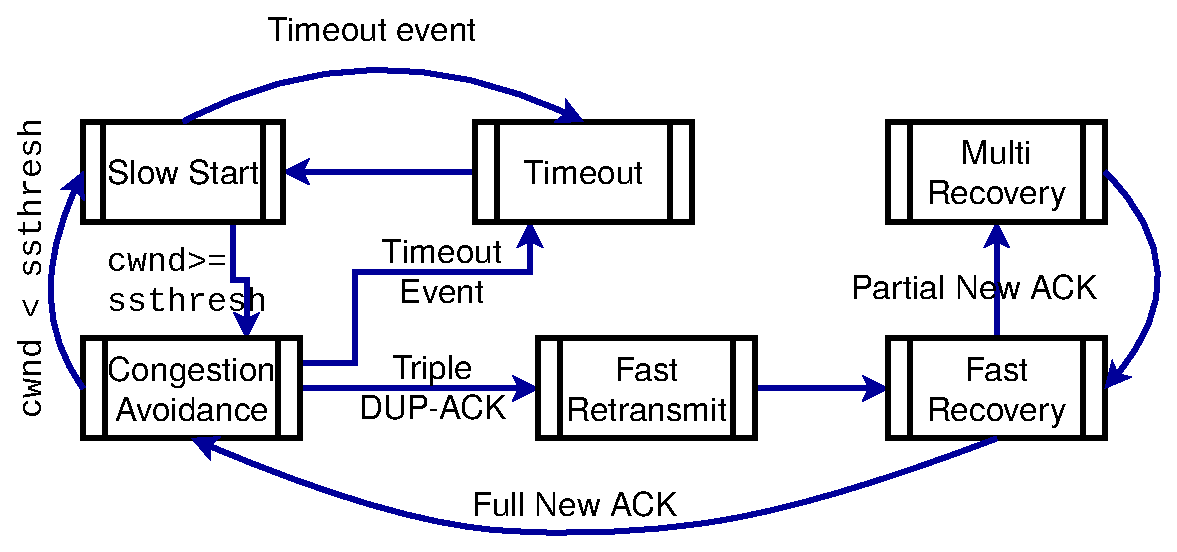
\includegraphics[width=0.8\linewidth]{img/cong_state_tran.eps}
	\caption{State transition diagram in Viscous congestion control algorithm.}
	\label{img:cong-state-tran}
\end{figure}

{\bf Slow Start}: It is similar to TCP (Tahoe, Reno or new-Reno) congestion control. Here, congestion window size ($cwnd$) gets doubled in every round trip time (RTT). To, emulate this effect, we increase $cwnd$ by 1MSS (maximum segment size) upon receiving successful acknowledgment (ACK). The {\it Slow Start} state continue until $cwnd$ reaches Slow Start Threshold ($ssthresh$). Initially $ssthresh$ set to a large value (we use one-forth of the sequence number space {\it i.e.} 16384). 
%So, upon receipent of a successful ACK, $$cwnd_i = cwnd_{i-1} + 1$$

{\bf Congestion Avoidance}: This state is also similar to TCP; in this state, a Viscous channel increases its $cwnd$ by 1MSS in every RTT. Again to emulate this effect, $cwnd$ is updated as $cwnd= cwnd + \frac{1}{cwnd}$ upon receiving successful ACK. The congestion avoidance state continues until the sender receives three duplicate ACKs (triple-DUP ACK) or when timeout event occurs. On triple-DUP ACK event, a Viscous channel immediately goes to {\it Fast Retransmit} and on timeout event, it moves to {\it Timeout} state.

{\bf Fast Retransmit}: In this state, Viscous channel immediately transmits the undelivered packet, and moves to {\it Fast Recovery} state. {\it Fast Retransmit} state is very brief, and it only transmits the missing/undelivered packets. Also, it sets $ssthresh$ to half the current $cwnd$ and mark the maximum sequence number that sent through the channel till now. This marked sequence number will be used in other states.

At this point we need to understand when Viscous sender transmit a packet. Viscous sender transmit a packet when ever there is a packet available in the buffer and $cwnd$ is lesser than flight size. Flight size is the number of packets that have been sent but not acknowledged till now.

{\bf Fast Recovery}: In this state, Viscous channel tries to send a new packet for every DUP-ACKs. When a channel receives a DUP-ACK, it means that the network can deliver further packets as the other end has received some packets. So, sender can transmit some packets. As this DUP-ACK does not decrease the flight size, sender need to increase the $cwnd$ to transmit extra packets. So, we increase $cwnd$ by 1MSS for every DUP-ACKs. It should be noted that, it is not effective increment of $cwnd$. Here we increase $cwnd$ just to send new packet as a response to DUP-ACK. We reset $cwnd$ as soon as {\it Fast Recovery} or {\it Multi Recovery} ends.

In Viscous, we uses a field header called {\tt orig-ack} in its packet. It contains the original packet number, which triggered a DUP-ACK at the receiver side. This field allows a Viscous channel to track the delivered packets at the receiver side like TCP SACK option, and sender don't have to retransmit the acknowledged packet again. During {\it Fast Recovery} state, sender expect to see a new ACK which acknowledges all the the packet it sent till it received last triple DUP-ACKs i.e. the marked sequence number in {\it Fast Retransmission} state. This type of ACK call full new ACK. It means there was only one missing packet. On the other hand, if it receives a new ACK which does not acknowledges all packet upto the mark sequence number, it is partial new ACK. It, means there are multiple packet loss happened the channel. When the sender receives a partial ACK in {\it Fast Recovery} state, channels moves to {\it Multi Recovery} state to recover other missing packets. This behavior is slightly different from TCP SACK option. In SACK option, sender send missing packets  only when retransmission timeout expires. In Viscous, sender can retransmit missing packets as soon as it received partial new ACK if retransmission timeout haven't expired yet.

{\bf Multi Recovery}: In this state, Viscous channel retransmit all the undelivered packets in the sender window. If it exhaust the undelivered packets in the sender window, it again moves to {\it Fast Recovery} state. We use this state to avoid timeouts for multiple packets when there is multiple packet loss in a single window. During this state, $cwnd$ does not change at all.

{\bf Timeout}: It is same as TCP timeout state. Whenever timeout occurs for a packets, Viscous channel moves to {\it Timeout} state. This is also very. In {\it Timeout} state, Viscous channel retransmit the packets and set $ssthresh$ to half of the current $cwnd$ and set $cwnd$ to 1. Immediately after that, Viscous channel moves to {\it SlowStart} state. Timeout event governs by Retransmission Timeout ($rto$) which is calculated as follows.

\begin{equation}
\begin{split}
rttvar &= (1-\beta) * rttvar + \beta * (srtt ~ rtt)\\
srtt &= (1-\alpha)*srtt + \alpha*rtt \\
rto &= srtt + \max(G, 4*rttvar) \\
\end{split}
\end{equation}

where $rtt$ is RTT measured by a single packet and $srtt$ is smoothed RTT. $\alpha$ and $\beta$ are smoothing parameter set to 0.8. $G$ is the granularity of the clock being used in the implementation. This values are similar to the ones set by Jacobson in \cite{Jacobson:1988:CAC:52325.52356,RFC2988}.





\section{Decoupling of Flow and Congestion Control}
As mentioned earlier, Viscous decouples congestion and flow control, where congestion control is associated with the channel layer, and flow control is associated with the flow layer. The flow control algorithm uses the receiver advertised window size ($rwnd$) to control the rate of traffic flows from the application, so that the traffic generation rate from the source application does not overshoot the traffic reception rate at the target application. The interesting design choice for Viscous is that if there is congestion in one of the paths among all the available ones, the traffic generation rate from the application may not need to be dropped down when other paths (or channels) have sufficient bandwidth. However, when congestion is severe (there is congestion in more than one paths), that feedback needs to be passed to the flow control module so that the application traffic generation rate can be shaped accordingly to avoid data overflow from the Viscous packet buffer. Therefore, we design the following approach for decoupled flow and congestion controls in Viscous. 
%Here we will try to find the relation between flow-control and congestion-control.

\subsection{Mesuring mean throughput achieved by a channel}
At first we try to model expected congestion window size ($cwnd$) in steady state condition for a single channel. We  follow the modeling provided in \cite{Padhye2000}. Here we assumes that in steady state, available bandwidth is almost constant. RTT varies only because of the queuing delay. Also, links are lossless and packets get dropped due to buffer overflow at the different queues i.e. packet loss are the signal for congestion in the path.

As mentioned in the earlier section, the congestion control algorithm has five states which are {\it Slow Start}, {\it Congestion Avoidance}, {\it Fast Retransmit}, {\it Fast Recovery}, {\it Multi Recovery} and {\it Timeout}. Among them {\it Fast Retransmit} and {\it Timeout} are very brief to affect anything to have any effect on the mean $cwnd$ however require to transmit the lost packets immediately.

\begin{figure}[!h]
	\centering
	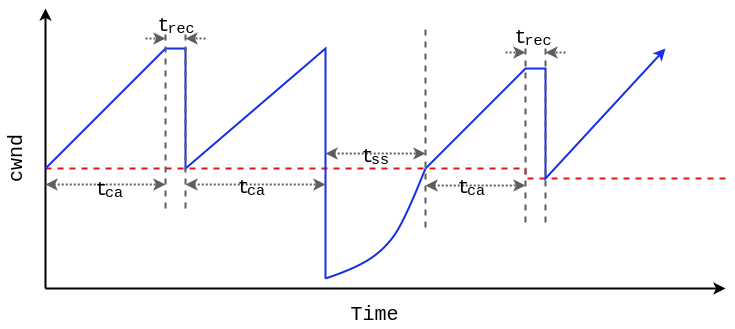
\includegraphics[width=\linewidth]{img/model/window_evolution}
	\caption{Theoretical steady state window evolution by the proposed congestion control algorithm.}
	\label{fig:cwnd-evo}
\end{figure}

In Fig.~\ref{fig:cwnd-evo}, we have shown $cwnd$ evolution in steady-state for a Viscous channel. Here, $cwnd$ starts from $ssthresh$ and the Viscous channel is in {\it Congestion Avoidance} state. $cwnd$ grows upto $cwnd_{max}$ for $t_{ca}$ duration till sender receives a three duplicate ACKs (DUP). Then it spends in {\it Fast Retransmission} state for a very brief time and moves to {\it Fast Recovery} state. It may happen that the Viscous channel moves to {\it Multi Recovery} state. However, there are no change in congestion window $cwnd$ until it get out of the recovery state. Total duration it have to spent in the recovery state for $t_{rec}$ time.

In steady-state, timeout may occur for some packets. In that case, the Viscous channel moves to {\it Slow Start} state and spends $t_{ss}$ duration before it moves to the {\it Congestion Avoidance} state. Now, let the probability of spending time at {\it Congestion Avoidance} state be $p_{ca}$ and probability of spending time at {\it SlowStart} state be $p_{ss}$.

\begin{equation} \label{eqn:cwnd_update}
cwnd_{i+1} = 	
\begin{cases}
 2 \times cwnd_{i} & \text{\it SlowStart} \\
 cwnd_{i} + 2 & \text{\it Congestion Avoidance} \\
 cwnd_{i} / 2 & \text{On three DUP ACK} \\
 1 & \text{On timeout event} 
\end{cases}
\end{equation}

Now, there are several way congestion window ($cwnd$) updates as per the Eqn.~\ref{eqn:cwnd_update}, i.e. it doubles the $cwnd$ per RTT during the {\it Slow Start} state and increases by 1 packet per RTT in the {\it Congestion Avoidance} state. Upon receipt of three duplicate ACKs, $cwnd$ set to half and after a timeout, it set $cwnd$ to 1.
Upon receipt of three duplicate ACKs, a Viscous channel spent some time in recovery state ({\it Fast Recovery} and {\it Multi Recovery}). During this period, effective $cwnd$ does not change. The Viscous channel stays in {\it Congestion Avoidance} state for $t_{ca}$ time, $t{rec}$ time in recovery state and $t_{ss}$ time in {\it Slow Start} state.


Now, the average congestion window ($cwnd$) during {\it Slow Start}($cwnd_{avg_{ss}}$), {\it Congestion Avoidance} ($cwnd_{avg_{ca}}$), and Recovery ($cwnd_{avg_{rec}}$) states are

\begin{equation}
\begin{split}
cwnd_{avg_{ss}} &= \frac{\int\limits_{0}^{t_{ss}} 2^x dx}{t_{ss}} \\
&= \frac{2^{t_{ss}}-1}{t_{ss} \times \ln{2}}
\end{split}
\end{equation}

\begin{equation}
\begin{split}
cwnd_{avg_{ca}} = ssthresh + \frac{1}{2}t_{ca}
\end{split}
\end{equation}

\begin{equation}
\begin{split}
	cwnd_{avg_{rec}} = t_{ca}+ssthresh
\end{split}
\end{equation}

Recovery state happens only after three duplicate ACKs, but not after a timeout. So, in the steady states, it is recovery state or {\it Slow Start} state after a {\it Congestion Avoidance} state. So, we need to find out the mean $cwnd$ for (a) {\it Congestion Avoidance} state followed by a recovery state (i.e. $cwnd_{avg_{ca+rec}}$) and for (b) {\it Congestion Avoidance} state followed by a {\it SlowStart} (i.e. $cwnd_{avg_{ca+ss}}$) (Fig.~\ref{img:cong-state-tran}).

\begin{equation}
\begin{split}
&cwnd_{avg_{ca+rec}} \\
&= \frac{cwnd_{avg_{ca}} \cdot t_{ca} + cwnd_{avg_{rec}} \cdot t_{rec}} {t_{ca} + t_{rec}} \\
&= \frac{\frac{1}{2} t_{ca}^2+ssthresh \cdot t_{ca} + (t_{ca}+ssthresh) \cdot t_{rec}}{t_{ca} + t_{rec}} \\
&= \frac{1}{2} \cdot \frac{t_{ca}^2}{t_{ca} + t_{rec}} + \frac{t_{ca} \cdot t_{rec}}{t_{ca} + t_{rec}} + \frac{2 \cdot ssthresh}{t_{ca} + t_{rec}}
\end{split}
\end{equation}

\begin{equation}
\begin{split}
cwnd_{avg_{ca+ss}} &= \frac{cwnd_{avg_{ca}} \cdot t_{ca} + cwnd_{avg_{ss}} \cdot t_{ss}} {t_{ca} + t_{ss}} \\
&= \frac{\frac{1}{2} t_{ca}^2+ssthresh \cdot t_{ca} + \frac{2^{t_{ss}}-1}{\ln{2} \cdot t_{ss}} \cdot t_{ss}}{t_{ca} + t_{ss}} \\
\end{split}
\end{equation}


We assume that the probability of occurrence of timeout is $p$ and probability of triple DUP is ($1-p$). So, the average congestion window $cwnd_{avg}$ for a single Viscous channel.
\begin{equation}
\begin{split}
cwnd_{avg} = p \cdot cwnd_{avg_{ca+ss}} + (1-p) \cdot cwnd_{avg_{ca+rec}}
\end{split}
\end{equation}

This is same for all the channel available in a Viscous connection. So, we can write that average congestion window size in steady state for $i^{th}$ channel is $cwnd_{avg_i}$.

Till now, we measured the time with respect to a RTT. Let us assume that the mean RTT of the channel $i$ is $rtt_{m_i}$. Then throughput $B_i$ of the channel is, 
\begin{equation}
B_i = \frac{cwnd_{avg_i}}{rtt_{m_i}}
\end{equation}


So, the overall throughput $\mathcal{B}$ of a Viscous connection is:
$$ \mathcal{B} = \sum_{i}^{} B_i = \sum_{i}^{} \frac{cwnd_{avg_i}}{rtt_{m_i}} $$


However, it is the maximum throughput we can get from the channel layer where there is no flow control applied. Now, if we consider Flow layer, our system looks like Fig.~\ref{fig:sys_que}. Here we have $n$ flows in flow layer. Scheduler collect data from flow as scheduling policy and bandwidth available at channel layer. There can be multiple channel in the system, each channel can transmit data reliably to a remote host.

\begin{figure}[!h]
	\centering
	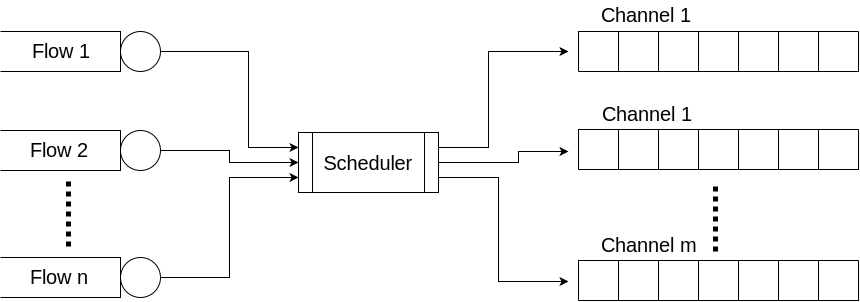
\includegraphics[width=\linewidth]{img/model/system_queue}
	\caption{Queuing diagram.}
	\label{fig:sys_que}
\end{figure}

\begin{algorithm*}[!ht]
	\SetKwFunction{findAllocation}{findAllocations}
	\nonl\findAllocation{$\mathcal{B}, \mathcal{X}, \mathcal{W}$}\\
	\KwData{$\mathcal{B} \gets \text{ available bandwidth}$ \\
				$\mathcal{X} \gets \{\mathcal{X}_1, \mathcal{X}_2 ... \mathcal{X}_n \}$ \\
				$\mathcal{W} \gets \{w_1, w_2 ... w_n\} $
				}
	\KwResult{$\mu \gets \{\mu_1, \mu_2 ... \mu_n\}$}
	\Indp
	\If{$|X| == 0$}{\Return{\{\}}}
	$\mu^s \gets \{\}$ //sets where $\mathcal{X}_i < \frac{w_i}{\sum_{\forall j}w_j} \mathcal{B}$\\
	$\mu^h \gets \{\}$ //sets where $\mathcal{X}_i \ge \frac{w_i}{\sum_{\forall j}w_j} \mathcal{B}$ \\
	\ForAll{$\mathcal{X}_i \in \mathcal{X}$}{
		$\mu_i \gets \frac{w_i}{\sum_{\forall j}w_j} \mathcal{B}$ \\
		\If{$\mu_i > \mathcal{X}_i$}{
			$\mu^s \gets \mu^s \cup \{\mathcal{X}_i\}$ \\
		}
		\Else{$\mu^h \gets \mu^h \cup \{\mu_i\}$}
	}
	\If{$|\mu^h| = |\mathcal{X}|$}{
		$\mu \gets \mu^h$ \\
		\Return $\mu$
	}
	\If{$|\mu^s| = |\mathcal{X}|$}{
		$\mu \gets \mu^s$ \\
		\Return $\mu$
	}
	
	$\mu \gets \mu^s$
	
	$\mathcal{B}' \gets \mathcal{B} - \sum_{ \mu_i \in \mu} \mu_i$ \\
	$\mathcal{X}' \gets \mathcal{X} \setminus \{\mathcal{X}_i | \forall_i \mu_i \notin \mu\}$ \\
	$\mathcal{W}' \gets \mathcal{W} \setminus \{w_i | \forall_i \mu_i \notin \mu\}$ \\

	$\mu \gets \mu\ \cup$ \findAllocation{$\mathcal{B}', \mathcal{X}', \mathcal{W}'$}\\
	\Return{$\mu$}
\caption{\label{algo:findTheBandwidth} Finding best bandwidth allocation based on the weights}
\end{algorithm*}


%\subsection{Scheduling}
Flow layer sends packets to the scheduler, and the scheduler schedules packets to the channels. The maximum arrival rate at the scheduler from the all flows can be $\mathcal{B}$ i.e. cumulative bandwidth of the channels. The scheduler schedules packets from $i^{th}$ flow with weight $w_i$. $w_i$ is an integer with minimum value 1. For rest of the part, we accumulated meaning of different symbols in Table~\ref{table:proofsymbols}.

\begin{table}
	\centering
	\begin{tabular}{|rl|}
		\hline
		$\mathcal{B} =$& Cumulative mean bandwidth available in all channels. \\
		$f_i =$& $i^{th}$ flow. \\
		$\mathcal{F} =$& Set of available flows in the viscous connection. \\
		$w_i =$& Weight of the flow $f_i$. It is integer with minimum value 1. \\
		$\mathcal{W} =$& Set of $w_i$ for all flows.\\
%		$\mathcal{P}_i=$& $\frac{w_i}{\sum_{i} w_i}$ \\
		$\lambda_i =$& Data generation rate at application for the flow $f_i$. \\
		$r_i =$& Maximum flow rate controlled receiver's window.\\
		$\mathcal{X}_i =$& $\min(r_i, \lambda_i)$\\
		$\mathcal{X} =$& Set of $\mathcal{X}_i$ for all flows.\\
		$\mu_i =$& Allocated bandwidth to flow $f_i$.\\
		$\mathcal{\mu} =$& Set of allocated bandwidth.\\
		\hline
	\end{tabular}
	\caption{\label{table:proofsymbols}List of symbols}
\end{table}

Each flow has two independent parameters, (a) data generation rate ($\lambda_i$) from the application and (b) flow rate ($r_i$) controlled by the receiver's window. So, a flow can send data at most $\mathcal{X}_i = \min(\lambda_i, r_i)$. The scheduler needs to allocate bandwidth $\mu_i$ from the available bandwidth $\mathcal{B}$ as per their weight $w_i$ i.e $\mu_i = w_i \cdot \mathcal{B}/\sum_{w_j}w_j$. The scheduler also do not want to keep channels under-utilized. In case, for some flow $f_i$, $\mathcal{X}_i < w_i \cdot \mathcal{B}/\sum_{w_j}w_j$, scheduler allocates $\mu_i = \mathcal{X}_i$ only and distributes surplus to other flow as per their weights. The bandwidth problem boils down to Proportional Fairness problem described by Kelly {\it et. al.} in \cite{Kelly1998}. Here we can describe our problem as the following optimization problem:

{\bf Objective:} $$\max \sum_{\forall i \in F} w_i \log \mu_i$$

{\bf Subjected to } $$\sum_{\forall_i \in F}\mu_i \le \mathcal{B}$$
{and} $$\mu_i \le \mathcal{X}_i \ \ \ \ \ \ \ \forall_i \in F$$

\subsection{Calculating a Feasible Allocation Vector}
Solution to this problem is as follows: $$\mu = F(\mathcal{B}, \mathcal{W}, \mathcal{X})$$

\begin{equation}
\label{eqn:formula}
F(\mathcal{B}, \mathcal{W}, \mathcal{X}) = 
\begin{cases}
\Phi & \text{if } |\mathcal{X}| == 0 \\ 

\{\mu_i = \frac{w_i}{\sum_{\forall j}w_j} \mathcal{B} | \forall_i\} 
& \text{if } \forall_i \mathcal{X}_i \ge \frac{w_i}{\sum_{\forall j}w_j} \mathcal{B} \\

\{\mu_i = \mathcal{X}_i\ | \forall_i \mathcal{X}_i \le \frac{w_i}{\sum_{\forall j}w_j} \mathcal{B} \} \cup F(\mathcal{B}', \mathcal{W}', \mathcal{X}') 
	& \text{Otherwise}
%	\ \ \hfill \text{if } \exists_i \mathcal{X}_i \le \frac{w_i}{\sum_{\forall j}w_j} \mathcal{B} \text{ and } \exists_i \mathcal{X}_i > \frac{w_i}{\sum_{\forall j}w_j} \mathcal{B}
\end{cases} \\
\end{equation}
While 
$$\mathcal{B}' = \mathcal{B} - \sum_{\forall_i \mathcal{X}_i \le \frac{w_i}{\sum_{\forall j}w_j} \mathcal{B}} \mathcal{X}_i$$
$$\mathcal{W}' = \mathcal{W} \setminus \{w_i | \forall_i \mathcal{X}_i \le \frac{w_i}{\sum_{\forall j}w_j} \mathcal{B} \}$$
$$\mathcal{X}' = \mathcal{X} \setminus \{\mathcal{X}_i | \forall_i \mathcal{X}_i \le \frac{w_i}{\sum_{\forall j}w_j} \mathcal{B}\})$$

%The Algorithm~\ref{algo:findTheBandwidth} provides a solution to the given recurrence in Eqn.~\ref{eqn:formula}.

\begin{theorem}
	The Algorithm~\ref{algo:findTheBandwidth} that solves eqn.~(\ref{eqn:formula}) gives the optimal solution for the optimization problem.
\end{theorem}

The allocation vector $\mu$ provided by the Algorithm~\ref{algo:findTheBandwidth}. As described in \cite{Kelly1998} by Kelly {\it et. al.}, $\mu$ is optimal iff for any feasible $\mu^*$, eqn~(\ref{eqn:proofeqn}) satisfy.

\begin{equation}
\label{eqn:proofeqn}
\sum_{\forall i} w_i \frac{\mu_i^* - \mu_i}{\mu_i} \le 0
\end{equation}

{\bf Proof}: The Algorithm~\ref{algo:findTheBandwidth} and Eqn.~(\ref{eqn:formula}) returns allocation $\mu$. It allocates available bandwidth among flows according to their weight and minimizes the bandwidth wastage. We can see that the algorithm allocates $\mathcal{X}_i$ to $i^{th}$ flow if possible and passes the surpass to next iteration to allocate accordingly based on the weights for rest of the flows. So, among $n$ flows, the algorithm allots $k$ flows to $\mathcal{X}_i$ and rest of the flows according to weight with remaining bandwidth. So, $$\mu = \{\mathcal{X}_1, \mathcal{X}_2, ... \mathcal{X}_k, \mu_{k+1}, ..., \mu_{n}\}$$ where $$\mu_i = \frac{w_{i}}{\sum_{j=k+1}^{n}w_j}(\mathcal{B} - \sum_{j=1}^{k}\mathcal{X}_i) \ \ \ \ for\ i=k+1,k+2,...,n$$

%Now, we want to proof $\mu$ is optimal using proof by contradiction. For the shake of contradiction, lets assume there exists some $\mu^* = \{\mu_i+\epsilon_i | \forall_i\}$ for which $$\sum_i w_i \frac{\mu_i^* - \mu_i}{\mu_i} > 0$$

To prove that our algorithm provides optimal solution, we have to prove three different cases depending on the value of $k$. These cases are ii) $k = 0$, ii) $0 < k < n$ and iii)$k = n$. These three cover all possible combination as it covers the range of $k$ ({\it i.e.} $0 \le k \le n$).

{\bf Case i:} When $k=0$, $\mu_i = \frac{w_i}{\sum_{j}w_j}\mathcal{B}$

Here, it is observed that $\sum_i \mu_i = \mathcal{B}$ and for any other feasible solution $\mu^* = \{\mu_i^* = \mu_i+\epsilon_i | \forall_i\}$, as per the constraints $\sum_i \mu_i^* \le \mathcal{B}$.

%\begin{equation}
%\begin{split}
%\sum_i \mu_i^* - \sum_i \mu_i \le& \ \mathcal{B} - \mathcal{B}\\
%\sum_i (\mu_i^* - \mu_i) \le& \ 0\\
%\sum_i \epsilon_i \le& \ 0
%\end{split}
%\end{equation}

%Now, 

\begin{equation}
\begin{split}
&\sum_i w_i \frac{\mu_i^* - \mu_i}{\mu_i} \\
&= \sum_i w_i \frac{\mu_i^* - \mu_i}{\frac{w_i}{\sum_{j}w_j} \mathcal{B}} \\
&= \sum_i  \frac{\sum_{j}w_j \cdot (\mu_i^* - \mu_i)}{\mathcal{B}} \\
&= \frac{\sum_{j}w_j}{\mathcal{B}} \sum_i (\mu_i^* - \mu_i)\\
&= \frac{\sum_{j}w_j}{\mathcal{B}} \left( \sum_i \mu_i^* - \sum_i \mu_i \right) \\
&\le 0 \\
& \omit \hfill \text{$\sum_i \mu_i^* \le \mathcal{B}$} \\
\end{split}
\end{equation}
$\mu$ is optimal for this case also.

{\bf Case ii:} When $0<k<n$
Here
\begin{equation}
\label{eqn:case3-1}
\begin{split}
\mu_i =& \mathcal{X}_i \\ & \omit\hfill \text{} i=1,2,...,k \\
\mu_i =& \frac{w_i}{\sum_{j=k+1}^{n} w_j} \left(\mathcal{B}-\sum_{j=1}^{k}\mathcal{X}_j\right) \\ & \omit\hfill \text{} i=k+1,k+2,...,n\\
\end{split}
\end{equation}

Our algorithm returns allocation $\mu$ where allocation for few flows are saturated (i.e. $\mu_i = \mathcal{X}_i$) and it is unsaturated for other flows. In every iteration, algorithm first try to distribute available bandwidth to every unsaturated flows. In this process, if any flows get saturated and have some surpass, algorithm go for next iteration and distribute the surpass among the unsaturated flow according to their weight. If surpass bandwidth in a iteration $x$ is $\mathcal{B}_{r_x}$ and the sum of weight of unsaturated flows in the same iteration $x$ is $\mathcal{W}_{s_x}$ then bandwidth allocation for $i^{th}$ flow which is unsaturated, in iteration $x$, will be $\mu_i = \min\left( \mu_i + w_i\frac{\mathcal{B}_{r_x}}{\mathcal{W}_{s_x}}, \mathcal{X}_i \right)$. So we can write that for a saturated flow $i$ 
\begin{equation}
\label{eqn:case3-2}
\begin{split}
\mu_i \le& w_i \left( \frac{\mathcal{B}}{w_{s_0}} + \frac{\mathcal{B}_{r_1}}{w_{s_1}} + \frac{\mathcal{B}_{r_2}}{w_{s_2}} + ... + \frac{\mathcal{B}_{r_m}}{w_{s_m}} \right) \\ 
& \omit\hfill \text{} i=1,2,...,k \\
\end{split}
\end{equation}

For a unsaturated flow $i$
\begin{equation}
\label{eqn:case3-3}
\begin{split}
\mu_i =& w_i \left( \frac{\mathcal{B}}{w_{s_0}} + \frac{\mathcal{B}_{r_1}}{w_{s_1}} + \frac{\mathcal{B}_{r_2}}{w_{s_2}} + ... + \frac{\mathcal{B}_{r_m}}{w_{s_m}} \right) 
\\ & \omit\hfill \text{} i=k+1,k+2,...,n\\
\end{split}
\end{equation}


We already know that $\sum_{i=1}^{n} \mu_i = \mathcal{B}$. We can also say that for any feasible allocation  $\sum_{i=1}^{n} \mu_i^* \le \mathcal{B}$. Now, $\mu$ has allocated bandwidth for $k$ flows to $\mathcal{X}_i$ which saturate there allocation. So, for any other feasible allocation, these $k$ flow can not be allocated more that. But, for rest of the flows, which have unsaturated allocation, can be allocated more. So, we can write that $\mu^* = \{\mu_i^* = \mu_i - \epsilon_i | i=1,2,...,k\}\cup\{\mu_i^* = \mu_i - \epsilon_i | i=k+1,k+2,...,n\}$

\begin{equation}
\label{eqn:case3-4}
\begin{split}
&\sum_{i=1}^{n} \mu_i^* - \sum_{i=1}^{n} \mu_i \le 0 \\
\implies & \sum_{i=1}^{k} \mu_i^* + \sum_{i=k+1}^{n} \mu_i^* - \left( \sum_{i=1}^{k} \mu_i + \sum_{i=k+1}^{n} \mu_i \right) \le 0 \\
\implies & \sum_{i=1}^{k} (\mu_i^* - \mu_i) + \sum_{i=k+1}^{n} (\mu_i^* - \mu_i) \le 0 \\
\implies & \sum_{i=1}^{k} -\epsilon_i + \sum_{i=k+1}^{n} \epsilon_i \le 0 \\
\end{split}
\end{equation}



Now, we can expand the Equation~(\ref{eqn:proofeqn}) as follows:

\begin{equation}
	\begin{split}
	& \sum_{i=1}^{n} w_i \frac{\mu_i^* - \mu_i}{\mu_i} \\
	=& \sum_{i=1}^{k} w_i \frac{\mu_i^* - \mu_i}{\mu_i} + \sum_{i=k+1}^{n} w_i \frac{\mu_i^* - \mu_i}{\mu_i} \\
	=& \sum_{i=1}^{k} w_i \frac{-\epsilon_i}{\mu_i} + \sum_{i=k+1}^{n} w_i \frac{\epsilon_i}{\mu_i}\\
	=& \sum_{i=1}^{k} w_i \frac{\epsilon_i}{-\mu_i} + \sum_{i=k+1}^{n} w_i \frac{\epsilon_i}{\mu_i}\\
	\le & \sum_{i=1}^{k} w_i \frac{\epsilon_i}{- w_i \left( \frac{\mathcal{B}}{w_{s_0}} + \frac{\mathcal{B}_{r_1}}{w_{s_1}} + \frac{\mathcal{B}_{r_2}}{w_{s_2}} + ... + \frac{\mathcal{B}_{r_m}}{w_{s_m}} \right)} \\ 
%	& \omit\hfill \text{$\epsilon_i \le 0 $  for $i=1,2...k$}\\
	& + \sum_{i=k+1}^{n} w_i \frac{\epsilon_i}{w_i \left( \frac{\mathcal{B}}{w_{s_0}} + \frac{\mathcal{B}_{r_1}}{w_{s_1}} + \frac{\mathcal{B}_{r_2}}{w_{s_2}} + ... + \frac{\mathcal{B}_{r_m}}{w_{s_m}} \right)} \\
	& \omit\hfill \text{from Eqn.~(\ref{eqn:case3-2}) \& Eqn.~(\ref{eqn:case3-3})} \\
	&= \frac{1}{\left( \frac{\mathcal{B}}{w_{s_0}} + \frac{\mathcal{B}_{r_1}}{w_{s_1}} + \frac{\mathcal{B}_{r_2}}{w_{s_2}} + ... + \frac{\mathcal{B}_{r_m}}{w_{s_m}} \right)} \left( \sum_{i=1}^{k} -\epsilon_i + \sum_{i=k+1}^{n} \epsilon_i\right)  \\
	&\le 0\\
	& \omit\hfill \text{from Eqn.~(\ref{eqn:case3-4})}\\
	\end{split}
\end{equation}

We can say that for any feasible allocation $\mu^*$.
\begin{equation}
\begin{split}
\sum_{i=1}^{n} w_i \frac{\mu_i^* - \mu_i}{\mu_i} \le 0
\end{split}
\end{equation}


{\bf Case iii:} When $k=n$, $\mu = \{\mu_i = \mathcal{X}_i | \forall_i\}$.

As per the constraint of the optimization problem, the maximum value of any $\mu_i$ is $\mathcal{X}_i$, so, for any other feasible $\mu^*$, $\mu_i^* \le \mathcal{X}_i$. 
\begin{equation}
\begin{split}
&\sum_i \mu_i^* \le \sum_i \mu_i \\
%\implies &\sum_i \mu_i^* - \sum_i \mu_i \le 0 \\
%\implies &\sum_i \left( \mu_i^* - \mu_i \right) \le 0\\
\implies &\sum_i w_i \frac{ \mu_i^* - \mu_i }{\mu_i} \le 0 \\
\end{split}
\end{equation} 
$\mu$ is optimal for case 1.
\\



So, the solution given by our algorithm is optimal for every cases and it allows us to utilize maximum available bandwidth available for at the channel layer.


\section{Viscous API Implementation}
We have implemented and tested Viscous protocol using C++ language in Linux kernel environment with \texttt{pthread}. We have made the Viscous implementation open-source, which is available at \url{https://github.com/abhimp/Viscous}. Further, due to space constraints, we are not able to provide the complete API details in this paper, and additional implementation details are available at \url{https://abhimp.github.io/Viscous/}.  
%The implementation details of Viscous is discussed next. 

%We have performed most of the experiment in network emulator Mininet and real network using raspberry pis. 

%Before we go deep into implementation, we will discuss the packet structure being used in our implementation.

\subsection{Viscous Packet Structure}
In Fig.~\ref{fig:packet_format}, we have depicted the packet structure used in our implementation. 
Each packet is divided into three parts -- a) mandatory header, b) variable length optional headers for additional information, and c) data region. The $28$ byte mandatory header has all the common fields required for the communication. The details of the mandatory fields are as follows. 
%
\begin{figure}[!t]
    \centering
    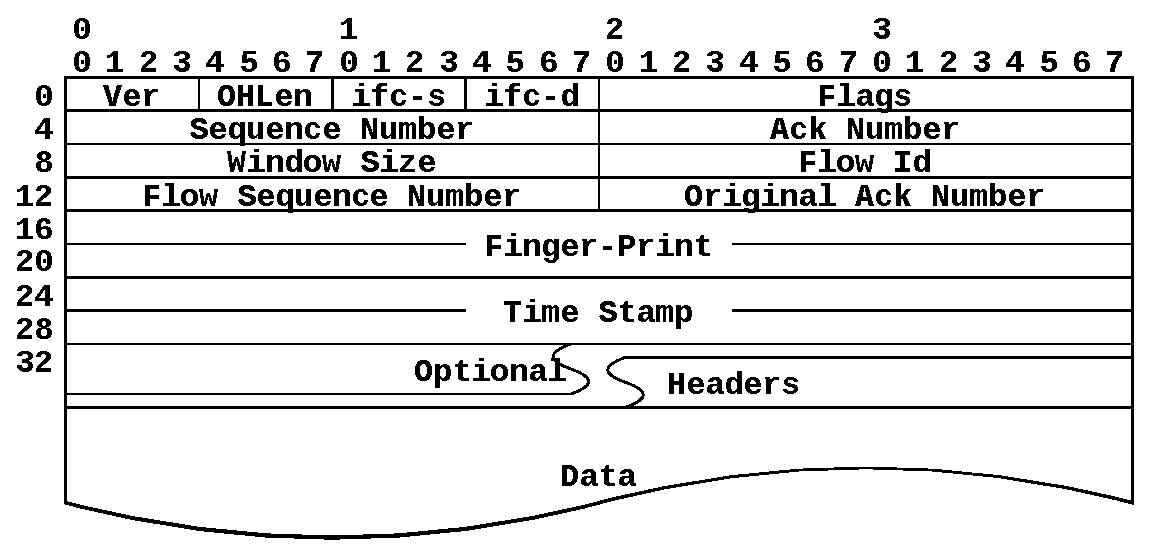
\includegraphics[width=0.85\linewidth]{img/Packet_format.eps}
    %\framebox[0.9\linewidth]{\input{img/Packet_format.tex}}
    \caption{Viscous packet header structure}
    \label{fig:packet_format}
\end{figure}
%\subsubsection{Mandatory header}
%Every packet starts with 28 bytes mandatory headers. It several fields. These fields are:
%\begin{itemize}
 
\noindent \textbf{Ver}: $4$ bits protocol version number. 
  %The current version is 1.
    
\noindent  \textbf{Optional Header Length(OHLen)}: We have optional headers of different sizes. This field helps decoder to understand how many optional headers need to be read before data section can be reached.
    
\noindent \textbf{ifc\_s}: 4 bit application defined source interface ID.
 
\noindent  \textbf{ifc\_d}: 4 bit application defined destination interface ID.

\hspace{3pt} Each application can use the device and list down the interface ids available. We assume that a device cannot have more than 15 interfaces. Interface ids start with 1. Interface id $0$ (zero) means it is not a valid interface. In our implementation, we use a pair of local and remote interface id as channel identifier. So, our implementation can support at most ($15\times15$) $225$ channels.
    
\noindent  \textbf{Flags}: We have used a set of boolean flags. It is similar to TCP. However Viscous need more flags as it is significantly different from TCP.
    
\noindent  \textbf{Sequence Number}:  Unlike TCP, the sequence number in Viscous is used to identify a packet rather than the byte stream. We use packet based sequence number because of two reasons -- a) packets are not created by channel handler; and b) as we multiplex multiple flows, it is easier to track a packet from a flow than a byte stream from a flow. Sequence numbers are used by channel handler to provide reliable communication between two applications. It can be noted that two channels can have same sequence number.
    
\noindent  \textbf{ACK Number}: It is cumulative acknowledgment number like TCP acknowledgment number. It denotes that the receiver has received contiguous packet up to this sequence number and it did not receive next packet until the time it was sent from the receiver.
    
\noindent \textbf{Window Size}: Receiver's advertise window. Channel does not use this window size. It is for flow handler.
    
\noindent  \textbf{Fingerprint}: It is Viscous client's unique ID generated by the server. Every packet includes this field except the initial synchronization packet for connection establishment. In Viscous, packets are discarded if this field is zero or if there is no connection matching this fingerprint (i.e. invalid fingerprint).
    
\noindent  \textbf{Flow ID}: Flow ID is an important field in a Viscous packet, which is used by the multiplexer to identify appropriate flow and to forward received packet accordingly.
    
\noindent  \textbf{Flow Sequence Number}: Each flow has its flow sequence number independent of the sequence number used by the channel. It requires at the flow layer to reorder the packets at the receiver side. We use packet based flow sequence number in Viscous, similar to the sequence number field.
    
\noindent  \textbf{Original ACK Number}: Viscous uses selective acknowledgment mechanism. When the receiver receives an out of order packet, it is supposed to send duplicate acknowledgment packet acknowledging the last conscious packet received. The receiver puts the original sequence number of the packet, which triggers the duplicate acknowledgment. This field gives sender an indication about packets received at the receiver side. So, the sender does not resend them again. It helps Viscous in reducing overall retransmission.
    
%    \item \textbf{Padding}: It is not a field.
    
\noindent  \textbf{Sent time-stamp}: When a sender sends a data packet, it includes the current Unix timestamp in microseconds ($\mu{s}$). When a receiver receives a data packets, it includes this timestamp with the ACK packet. It helps the sender in measuring the RTT more accurately.

\subsection{Modules and Layers in Viscous}
Viscous follows a modular architecture as shown in Fig.~\ref{fig:ModularDiagram}. The various modules in Viscous are as follows. 

\subsubsection{Application}
An application is the users' application that uses Viscous library. 


\subsubsection{Flow Handler}
In Viscous, an application directly sends data to this module and receives from it. Flow handler packetizes the raw data from the application and sends packets to the lower layer for further processing. It does not need to store any outgoing packets, as the channel layer ensures the reliability. It only keeps track of the packets that it sends, to control the flow rate. Viscous uses a sliding window based flow control mechanism based on the receiver advertised window size.
The flow handler also reorders the out of order packets that it receives from the lower layer. There is a receive buffer that stores all the out of order packets. This buffer is an array of packets. The first index of this packet array point to the next expected packet sequence. Whenever the flow handler receives one or more contiguous packets from the expected sequence, it delivers the data from those flows to the application. In Viscous, there is one independent flow handler instance for each of the flows.

\subsubsection{Multiplexer}
The multiplexer is responsible for multiplexing the outgoing packets from multiple flows and forwarding them to the packet scheduler. It is also responsible for demultiplexing incoming packets and forwarding them to appropriate flow handler. 

\begin{figure}[!t]
	\centering
	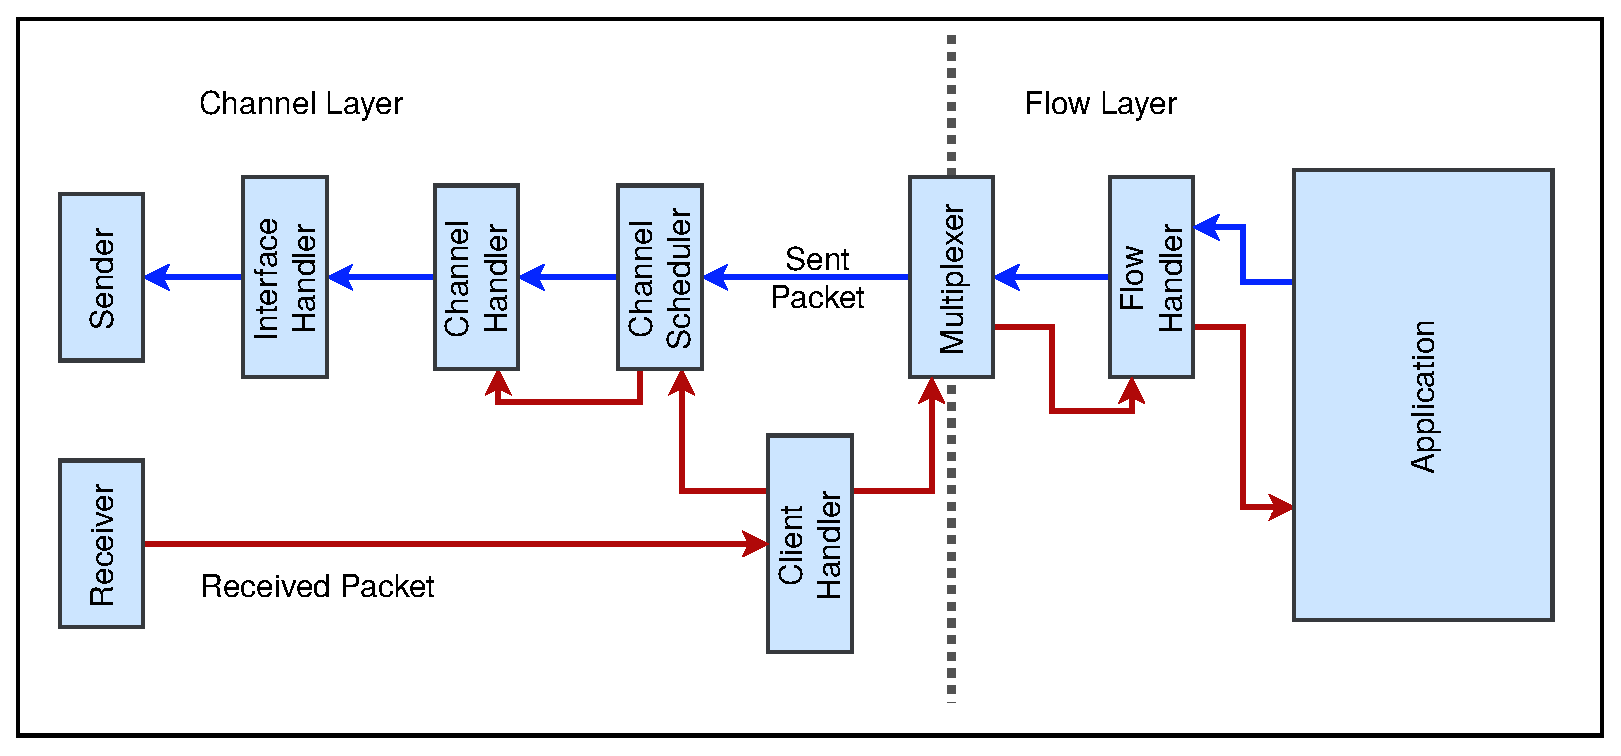
\includegraphics[width=.9\linewidth]{img/ModularDiagram}
	\caption{Internal packet and data flow diagram}
	\label{fig:ModularDiagram}
\end{figure}


\subsubsection{Client Handler}
Client handler is the manager of Viscous protocol API. 
For incoming packets, it checks the packet validity using the fingerprint generated during the connection establishment. 
After validation, it forwards each incoming packet to the {\em Channel Handler} via {\em Channel Scheduler} for further handling and processing for congestion control algorithm. 

\subsubsection{Channel Scheduler}
It schedules the outgoing packets to one of the channels. As mentioned earlier, we use \texttt{ACK} driven channel scheduling. Whenever a channel is ready to send packets, it asks the {\em Channel Scheduler} for new packets to be sent. A smart scheduler can decide which packet to be sent through a channel based on its algorithm to achieve high throughput with lower latency.


\subsubsection{Channel Handler}
Channel handler is responsible for reliable communication and congestion control in the network. We have discussed the congestion control algorithm in detail in section \ref{section:congestion_control}.

%In the Viscous implementation, we use the TCP New Reno congestion control~\cite{RFC2582} algorithm with the following modifications. In Viscous, the channel handler handles packets, not TCP like byte streams. So, we use packet based sequence number because it is easier to track a packet from a flow than a byte stream from a flow when we multiplex multiple flows. Further, in the Viscous congestion control, each \texttt{ACK} contains the sequence number of the packet for which this acknowledgment is triggered. This gives a similar effect as TCP selective acknowledgment (\texttt{SACK})~\cite{RFC2018} mechanism. Further, as flows are multiplexed, we have modified the fast recovery phase describe in RFC2581~\cite{RFC2582} with \texttt{SACK} modifications. After receiving the first partial new \texttt{ACK}, the channel handler sends all the unacknowledged (via \texttt{SACK} or original \texttt{ACK} in the packet header) packets up to the received acknowledgment number for each duplicate \texttt{ACK}. This modification reduces retransmissions due to timeout events when a series of packets get lost in the network.

\subsection{Mobility}
In our implementation, we have implemented Individual mobility for both the client and the server side. We consider the changes in network interface as external event. It was difficult to capture those events automatically from the application itself. So, for now we use a hack to catch those event. A Viscous application creates a {\it named fifo} in a predefined path (configurable via environment variable) to interact with other processes. There is a tool name NetworkManager available in most linux system can successfully capture all kind of events related to network interface in a  device. It also run various {\tt bash} script from the {\tt /etc/network} directory. We take advantage of this tool and put two scripts in the directory. One script runs when some network interface gets connected and another script runs whem a interface gets disconnected. These script passes this information to all the Viscous applications running in the device via the {\it name fifo}. This is a hack and we are working on the more generic way to capture the events.

%In our implementation, we have implemented Individual mobility for both the client and server side. We consider change in network interface as external event. To generate this event, we take help from NetworkManager tool available in most of the Linux distribution. Every time a interface gets connected or disconnected, NetworkManager run different script from {\tt /etc/network} directory. We take advantage of this behavior. We put few extra scripts there to pass those events to Viscous application via {\it named fifo} created by the application in predefined path. In the implementation, viscous library creates a {\it named fifo} in a predefined path and try read information in that fifo.




%\section{Experimental Evaluation}

To evaluate the performance of Viscous, we compare the Viscous with popular transport protocols MPTCP, MPQUIC, TCP and QUIC with different network configurations. We use the Mininet platform to perform most of our experiments. The mininet provides capability of generating different type of network topology with different network conditions in a single system and run any existing real network application on the Mininet generated network. We also performs few experiments on physical network using Raspberry Pi board.

For the Mininet based experiments, we use a computer with 8GB RAM, 4 core GenuineIntel i5-4590 CPU with 3.30 GHz clock frequency. It is equipped with Ubuntu 16.04.1 operating system with Linux kernel version 4.4.70 with the MPTCP v0.92 and the Mininet 2.2.2. For the Rapsberry pi setup, we use Raspberry Pi model 3.
To compare with the QUIC and the MPQUIC, we use golang implementation of the MPQUIC by Conick {\it et. al.}\cite{mpquic-measure} which is a extension of golang implementation of the QUIC\cite{quic-go}.

In rest of this section, we will produced different experiments and analysis of their results.

\begin{figure}
	\centering
	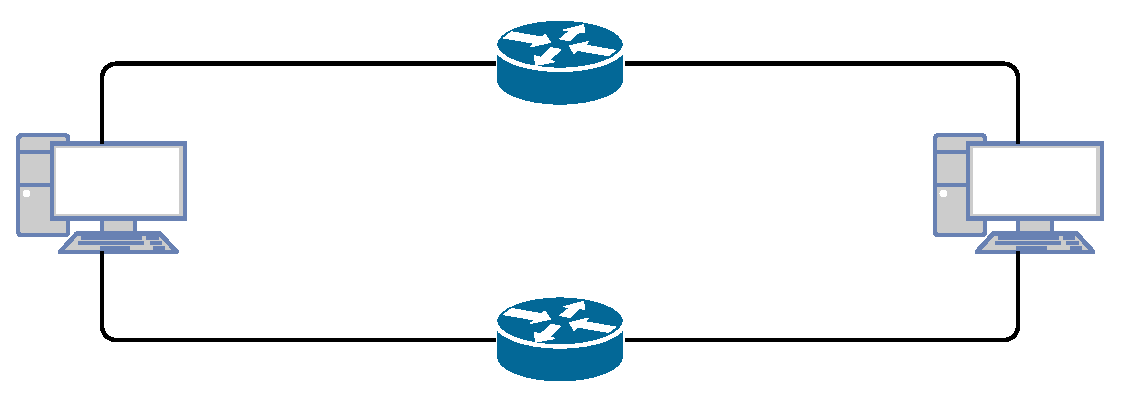
\includegraphics[width=\linewidth]{img/aggregation.eps}
	\caption{\label{fig:aggregation_dia}Network used to find aggregative benefit}
\end{figure}

\begin{table}[h]
	\centering
	\begin{tabular}{l||c|c||c|c}
		%		\hline
		& \multicolumn{2}{c||}{Low-BDP} & \multicolumn{2}{c}{High-BDP}\\
		\hline
		\hline
		Capacity [Mbps] & 0.1 & 100 & 0.1 & 100 \\
		\hline
		Propagation delay [ms] & 0 & 50 & 0 & 400 \\
		\hline
		Queuing [ms] & 0 & 100 & 0 & 2000 \\
		\hline
		Loss rate [\%] & 0 & 2.5 & 0 & 2.5 \\
		%		\hline
	\end{tabular}
	\caption{\label{tbl:noloss_param}Scenario used}
\end{table}

\begin{equation} \label{eqn:agre_benefit}
Bes(S) = 
\begin{cases}
\frac{G_v - G_p^{max}}{G_v - G_v^{max}} & \text{if} G_v > G_V^{max} \\
\frac{G_v - G_p^{max}}{G_v^{max}} & \text{otherwise}
\end{cases}
\end{equation}

\subsection{Measuring aggregated benefit}
To compare Viscous with other protocol in various network conditions, we perform similar experiment performed by \cite{mpquic-measure,Paasch:mptcp:compare}. We perform these experiments with various number of scenario by changing basic network parameters {\it e.g.} link bandwidth, RTT, queuing delay and packet loss rate. These experiments are performed using simple topology shown in Fig.~\ref{fig:aggregation_dia} with the help of Mininet network emulator. We run experiments on 143 scenario generated using WSP	space filling algorithm described in \cite{wspalgo} from configuration space described in Table~\ref{tbl:noloss_param}. Three experiment performed on each scenario for each protocols. We run experiments on TCP and QUIC for both the paths and compared with best performance. We also observed that the MPTCP depends on initial path selection, so we run experiments with MPTCP for both the path and compared with best and worst initial path performance. We considered GoodPut as the metric of performance. In each of these experiments, we send 50 back-to-back request-response over a single thread. The client request for a data-size to server and the server transfer the requested amount of data to client. We vary response size with a exponential distribution with mean 25KB\footnote{We decided 25KB as our initial observation with rich website yeld mean response size near 25KB.} payload.

To measure aggregative benefit, we followed modified equation provided in \cite{Kaspar:2012:MAH:2206765.2206770,Paasch:mptcp:compare,mpquic-measure}
as Equation~\ref{eqn:agre_benefit}. Here we measure the benefit of using Viscous instead of other protocol for a given scenario $S$. Here $G_v$ is the mean GoodPut found in all experiments using Viscous for the scenario $S$, $G_p^{max}$ is the max of mean GoodPut found in each path for single path protocol while $G_p^{max}$ is mean GoodPut achieved by a multipath protocol. The value of $Ben(S)$ is in between -1 to 1, while -1 mean GoodPut of other protocol is twice good as Viscous while 1 mean, GoodPut of other protocol is 0, and if $Ben(S)$ is 0, other protocol perform exactly same as Viscous. In Fig.~\ref{fig:benefit} and Fig.~\ref{fig:benefit-high}, we depicted the results of this experiment.

\begin{figure}
	\captionsetup[subfigure]{}
	\begin{center}
		\subfloat[\label{fig:benefit-box} Benefit of Viscous over other transport different protocol]{
			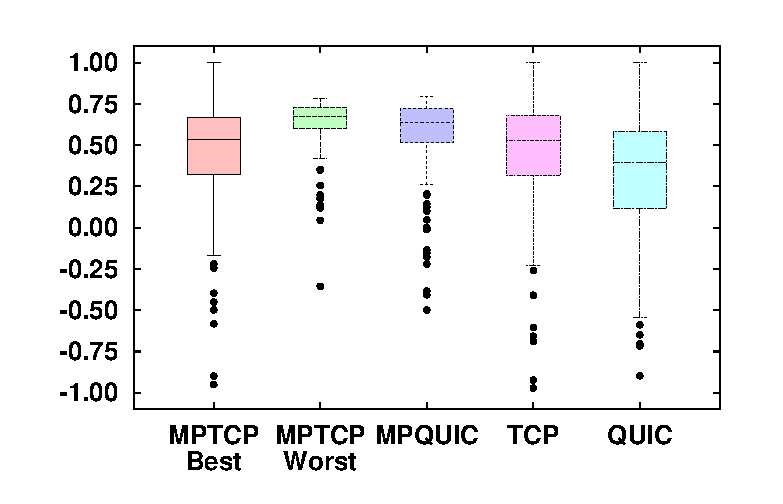
\includegraphics[width=.49\linewidth]{img/lowbdp-lossless/lowbdpnoloss_benefit.eps}
		}
		\subfloat[\label{fig:benefit-cdf} CDF of benefit of Viscous over other transport different protocol]{
			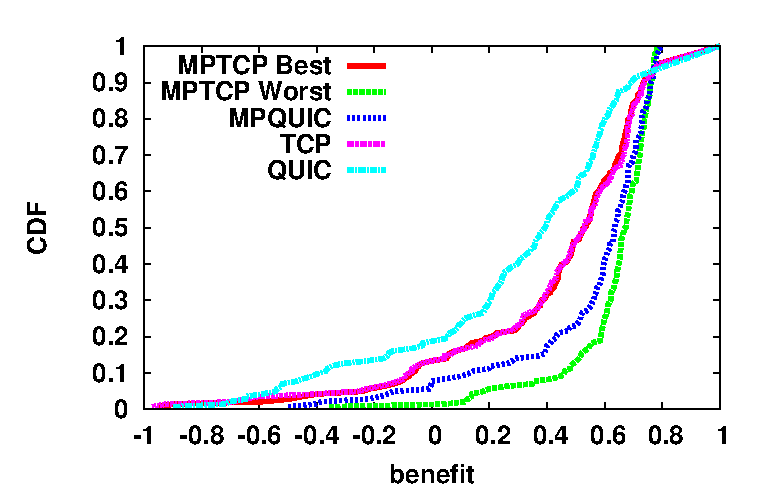
\includegraphics[width=.49\linewidth]{img/lowbdp-lossless/lowbdpnoloss_cdf.eps}
		}
		\caption{\label{fig:benefit}Experimental results on lossless low BDP channels}
	\end{center}
\end{figure}

We can see that the Viscous is performing better than all the other protocols. It can be understood that, the TCP and the MPTCP aren't performing good enough because they need to go through slow-start phase for every request. However it was not easy to find out the performance degradation of the QUIC or the MPQUIC. After taking close look to we found that congestion window have a limiting factor of 3.5MB in case of QUIC and MPTCP. This limiting factor is reducing the speed for the QUIC and MPQUIC while the Bandwidth or the RTT of the link is little higher. However, we kept no such limiting factor as speed is much more precious, the Viscous can have $cwnd$ size as high as the BDP for a channel.

\begin{figure}
	\captionsetup[subfigure]{}
	\begin{center}
		\subfloat[\label{fig:benefit-box-high} Benefit of Viscous over other transport different protocol]{
			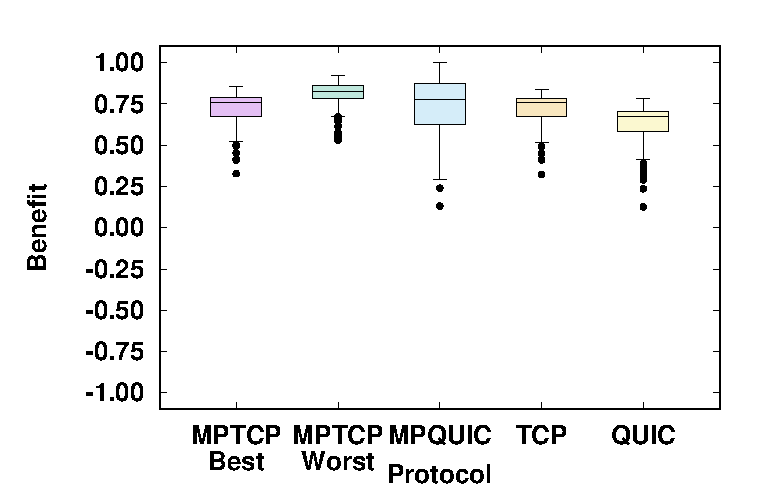
\includegraphics[width=.49\linewidth]{img/highbdp-lossless/highbdpnoloss_benefit.eps}
		}
		\subfloat[\label{fig:benefit-cdf-high} CDF of benefit of Viscous over other transport different protocol]{
			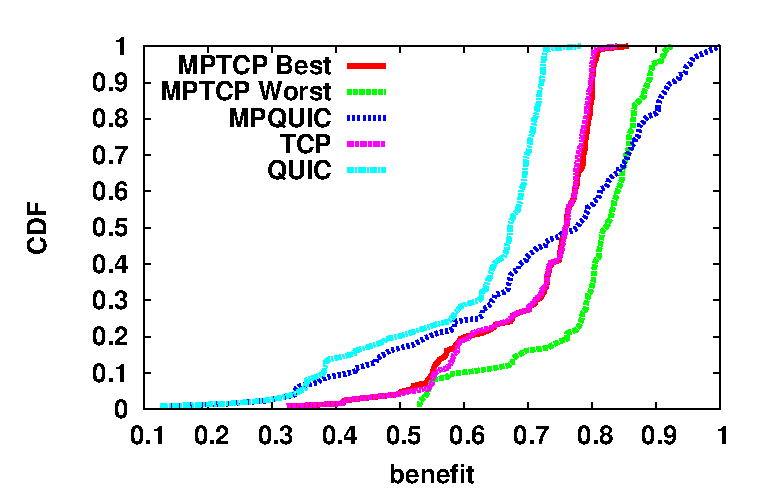
\includegraphics[width=.49\linewidth]{img/highbdp-lossless/highbdpnoloss_cdf.eps}
		}
		\caption{\label{fig:benefit-high}Experimental results on lossless high BDP channels}
	\end{center}
\end{figure}


%======================================
% place holder for experiments on lossy channels
%======================================
\begin{figure}
	\captionsetup[subfigure]{}
	\begin{center}
		\subfloat[\label{fig:benefit-box-lossy} Benefit of Viscous over other transport different protocol]{
			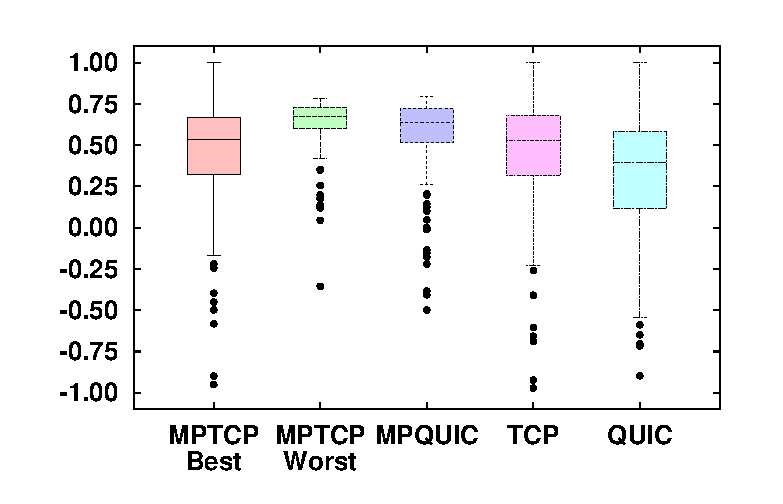
\includegraphics[width=.49\linewidth]{img/lowbdp-lossless/lowbdpnoloss_benefit.eps}
		}
		\subfloat[\label{fig:benefit-cdf-lossy} CDF of benefit of Viscous over other transport different protocol]{
			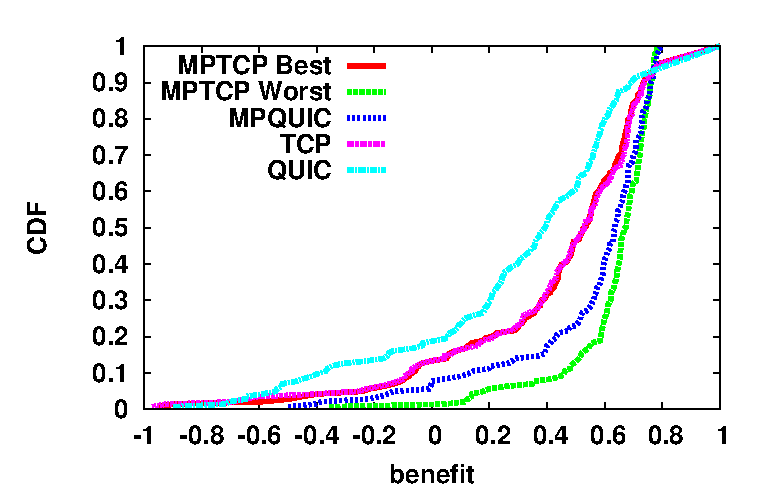
\includegraphics[width=.49\linewidth]{img/lowbdp-lossless/lowbdpnoloss_cdf.eps}
		}
		\caption{\label{fig:benefit-lossy}(\noteam{placeholder})Experimental results on lossy low BDP channels}
	\end{center}
\end{figure}

\begin{figure}
	\captionsetup[subfigure]{}
	\begin{center}
		\subfloat[\label{fig:benefit-box-high-lossy} Benefit of Viscous over other transport different protocol]{
			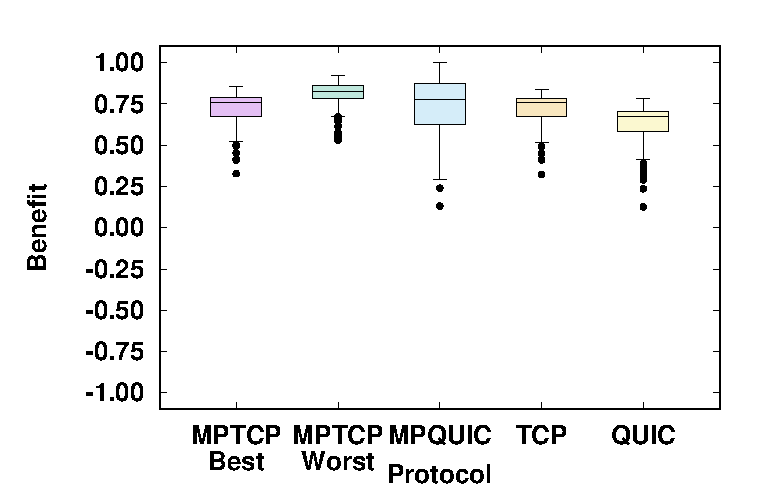
\includegraphics[width=.49\linewidth]{img/highbdp-lossless/highbdpnoloss_benefit.eps}
		}
		\subfloat[\label{fig:benefit-cdf-high-lossy} CDF of benefit of Viscous over other transport different protocol]{
			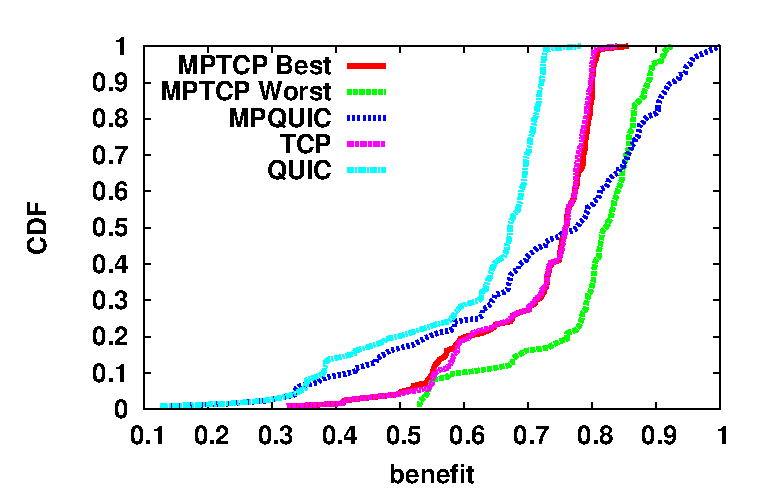
\includegraphics[width=.49\linewidth]{img/highbdp-lossless/highbdpnoloss_cdf.eps}
		}
		\caption{\label{fig:benefit-high-lossy}(\noteam{placeholder})Experimental results on lossy high BDP channels}
	\end{center}
\end{figure}

%======================================
% place holder for experiments on lossy channels
%======================================

\begin{figure*}[h]
	\captionsetup[subfigure]{}
	\begin{center}
		\subfloat[\label{fig:rocketfuel_time_5_20}Delay=5ms \#threads=5]{
			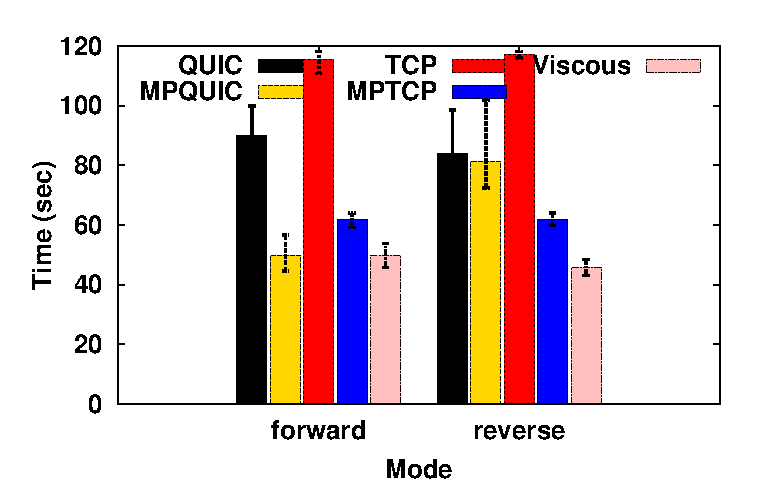
\includegraphics[width=0.24\linewidth]{img/rocketfuel/tymdiff-5-5.eps}
		}
		\subfloat[\label{fig:rocketfuel_time_10_5}Delay=10ms \#threads=5]{
			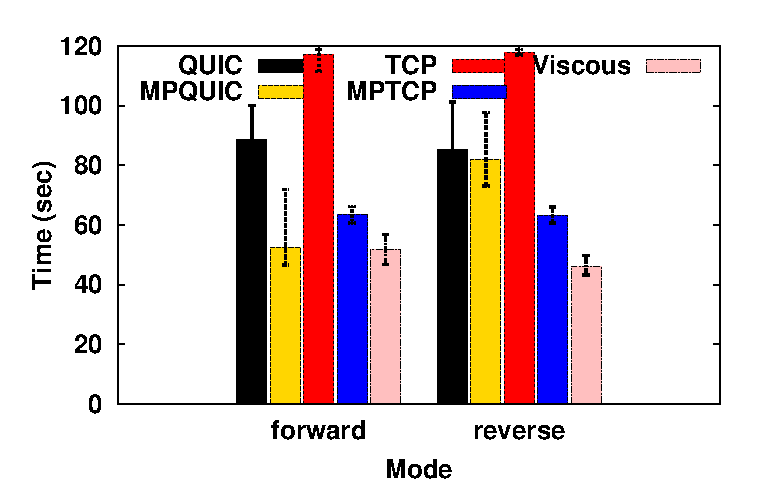
\includegraphics[width=0.24\linewidth]{img/rocketfuel/tymdiff-10-5.eps}
		}
		\subfloat[\label{fig:rocketfuel_time_10_20}Delay=10ms \#threads=20]{
			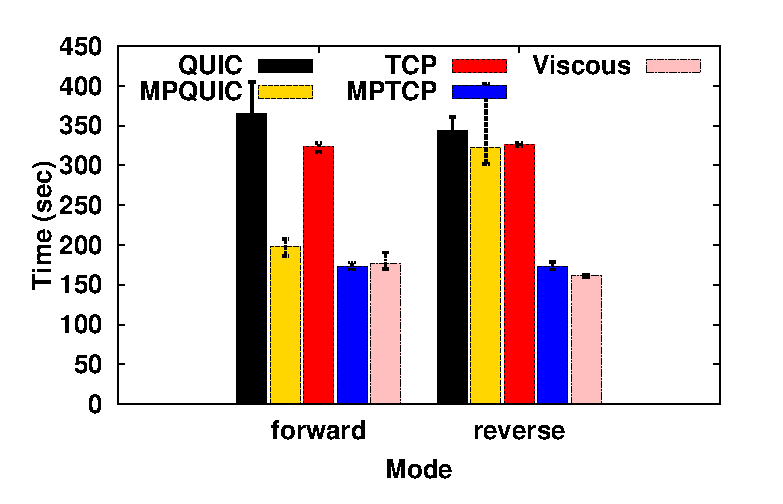
\includegraphics[width=0.24\linewidth]{img/rocketfuel/tymdiff-10-20.eps}
		}
		\subfloat[\label{fig:rocketfuel_time_20_20}Delay=20ms \#threads=20]{
			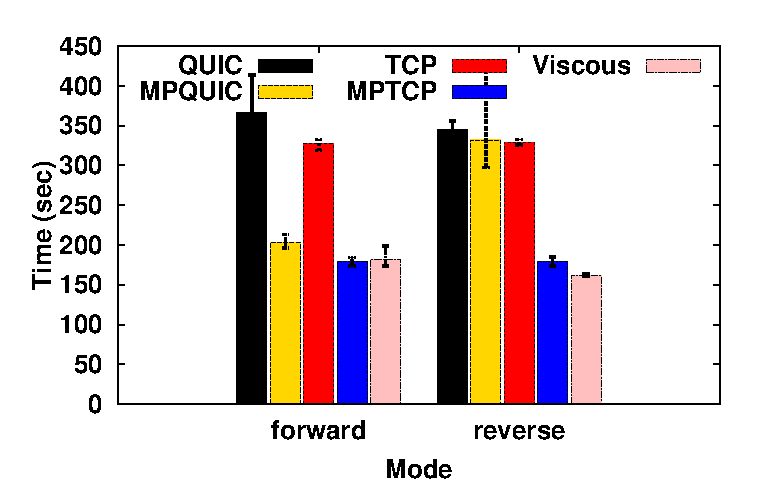
\includegraphics[width=0.24\linewidth]{img/rocketfuel/tymdiff-20-20.eps}
		}
		\caption{\label{fig:rocketfuel_time}Average average flow completion time over Rocketfuel topology}
	\end{center}
\end{figure*}


\begin{figure*}[h]
	\captionsetup[subfigure]{}
	\begin{center}
		\subfloat[\label{fig:rocketfuel_goodput_5_20}Delay=5ms \#threads=5]{
			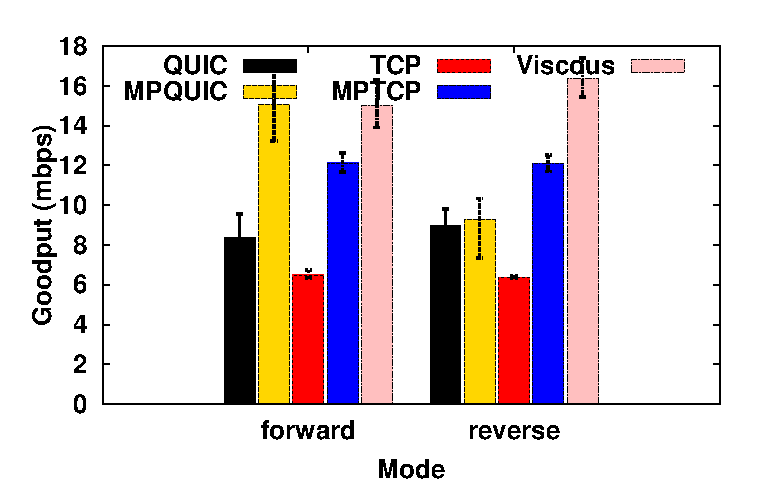
\includegraphics[width=0.24\linewidth]{img/rocketfuel/goodPut-5-5.eps}
		}
		\subfloat[\label{fig:rocketfuel_goodput_10_5}Delay=10ms \#threads=5]{
			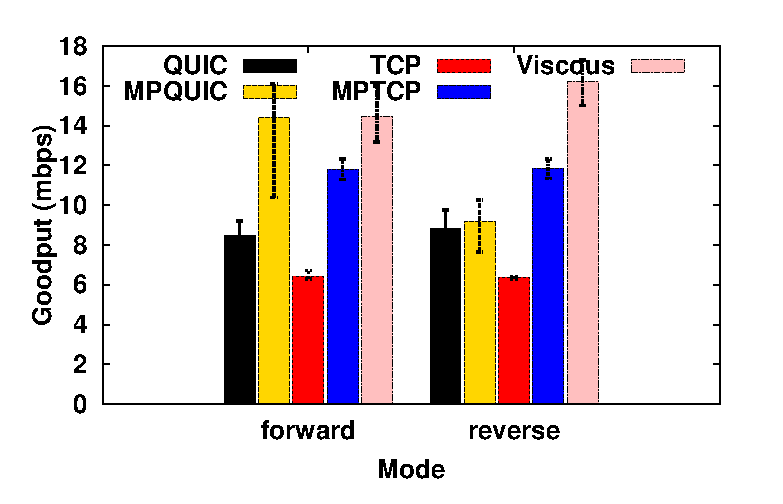
\includegraphics[width=0.24\linewidth]{img/rocketfuel/goodPut-10-5.eps}
		}
		\subfloat[\label{fig:rocketfuel_goodput_10_20}Delay=10ms \#threads=20]{
			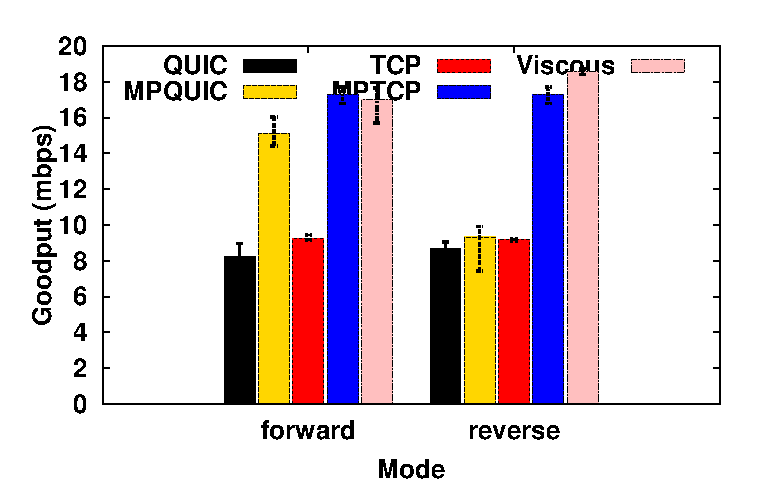
\includegraphics[width=0.24\linewidth]{img/rocketfuel/goodPut-10-20.eps}
		}
		\subfloat[\label{fig:rocketfuel_goodput_20_20}Delay=20ms \#threads=20]{
			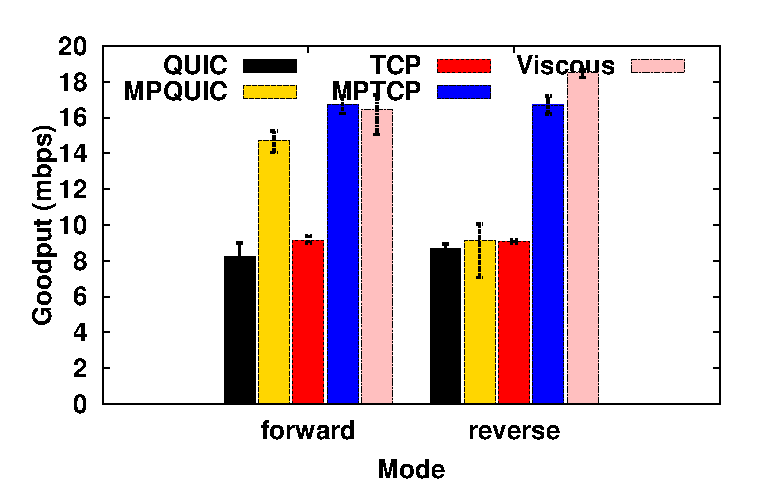
\includegraphics[width=0.24\linewidth]{img/rocketfuel/goodPut-20-20.eps}
		}
		\caption{\label{fig:rocketfuel_goodput}Average GoodPut over Rocketfuel topology}
	\end{center}
\end{figure*}

\subsection{Performance on overlapped path with RocketFuel topology}
The RocketFuel topology is a standard topology generated by using {\tt traceroute} from different locations all over the globe to different servers. We take a topology with 29 different networks connected via 15 routers. We place 14 host inside different networks. Among these 14 hosts, we connect 7 hosts with two different networks (we call it client host) and other 7 hosts with a single network (server host). So, there are 7 pair of server-client host. In this topology we use 3 different bandwidth for different links i.e. core link, server link, and client link. A core links connects a switch with a router with 100mbps bandwidth and 3ms delay, a server link connects a server and a switch with 50mbps bandwidth and 2ms delay. We keep 10mbps bandwidth for client link connecting a client host and a switch while varying the delay over different experiment.

In experiments, we sent data from each server host to their dedicated client host using different protocols (Viscous, QUIC, MPQUIC, TCP and MPTCP) and other way around. We call forward experiment when we send traffic from server host to client host and reverse experiment when we send data from client host to server host.

In this experiment, we vary client link delay and number of simultaneous thread. Then we send 50 back-to-connection through each thread with payload varied using exponential distribution with mean payload size 250kB. 


\begin{figure}
	\centering
	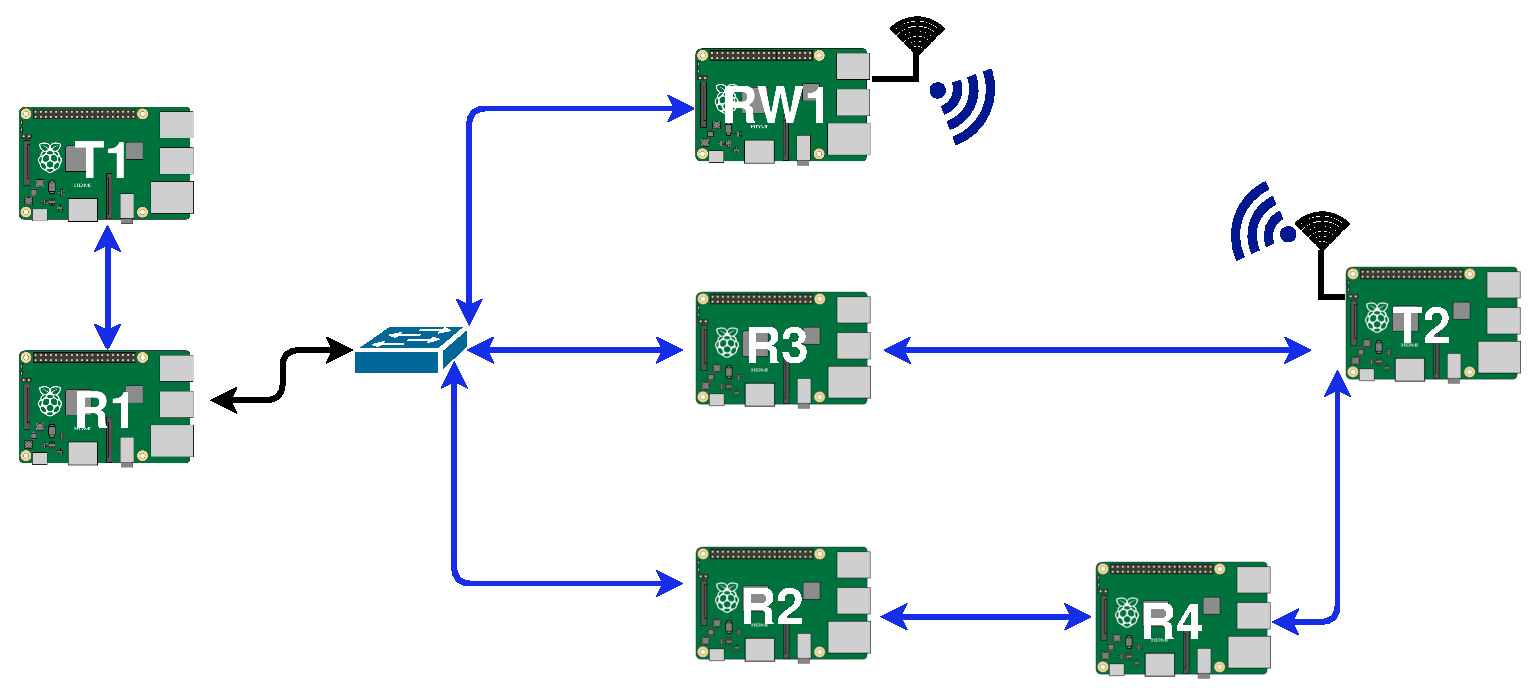
\includegraphics[width=.9\linewidth]{img/mobility/demo-Diagram.eps}
	\caption{\label{fig:mobility_diagram}Raspberry pi setup to test the mobility of viscous}
\end{figure}


\begin{figure*}[h]
	\centering
	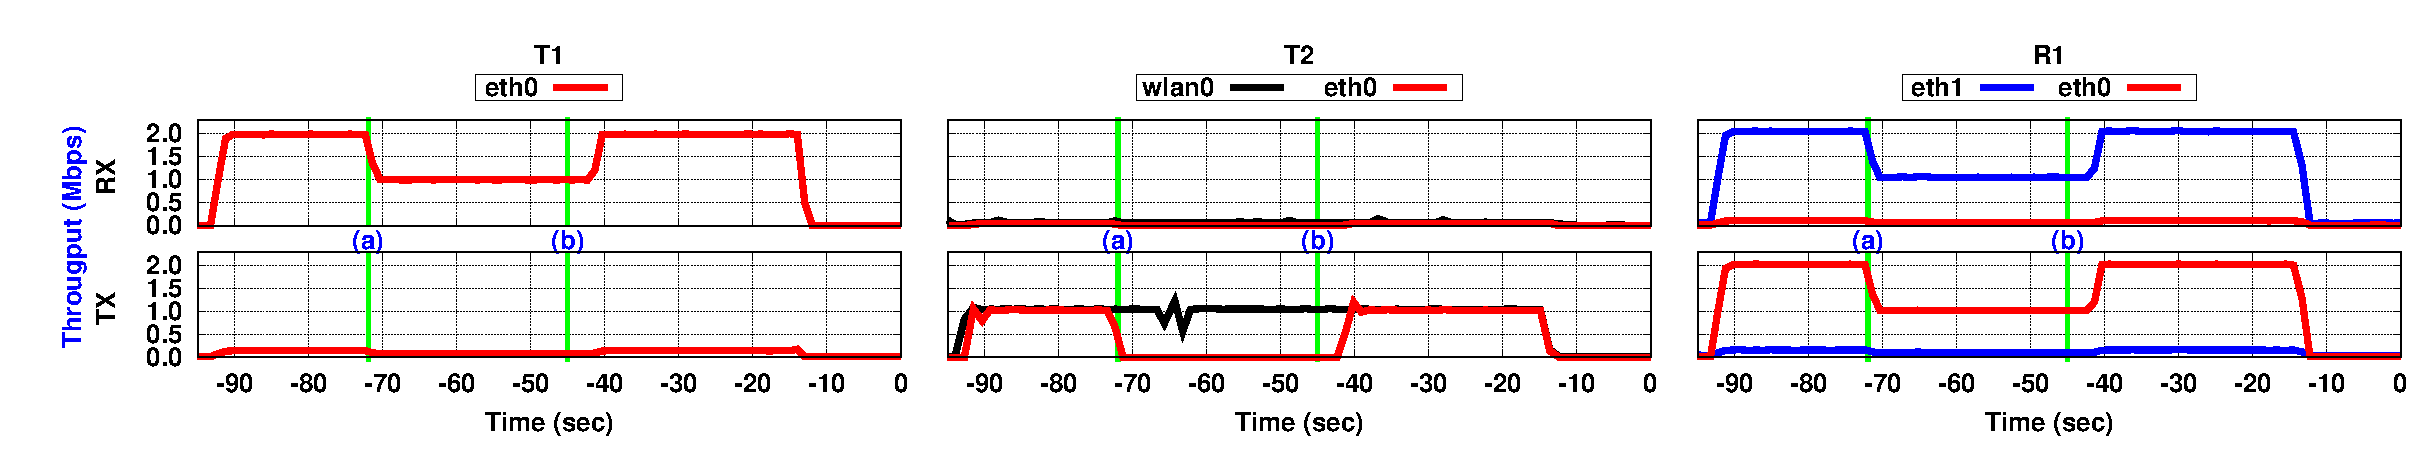
\includegraphics[width=\linewidth]{img/mobility/T1-T2-R1.eps}
	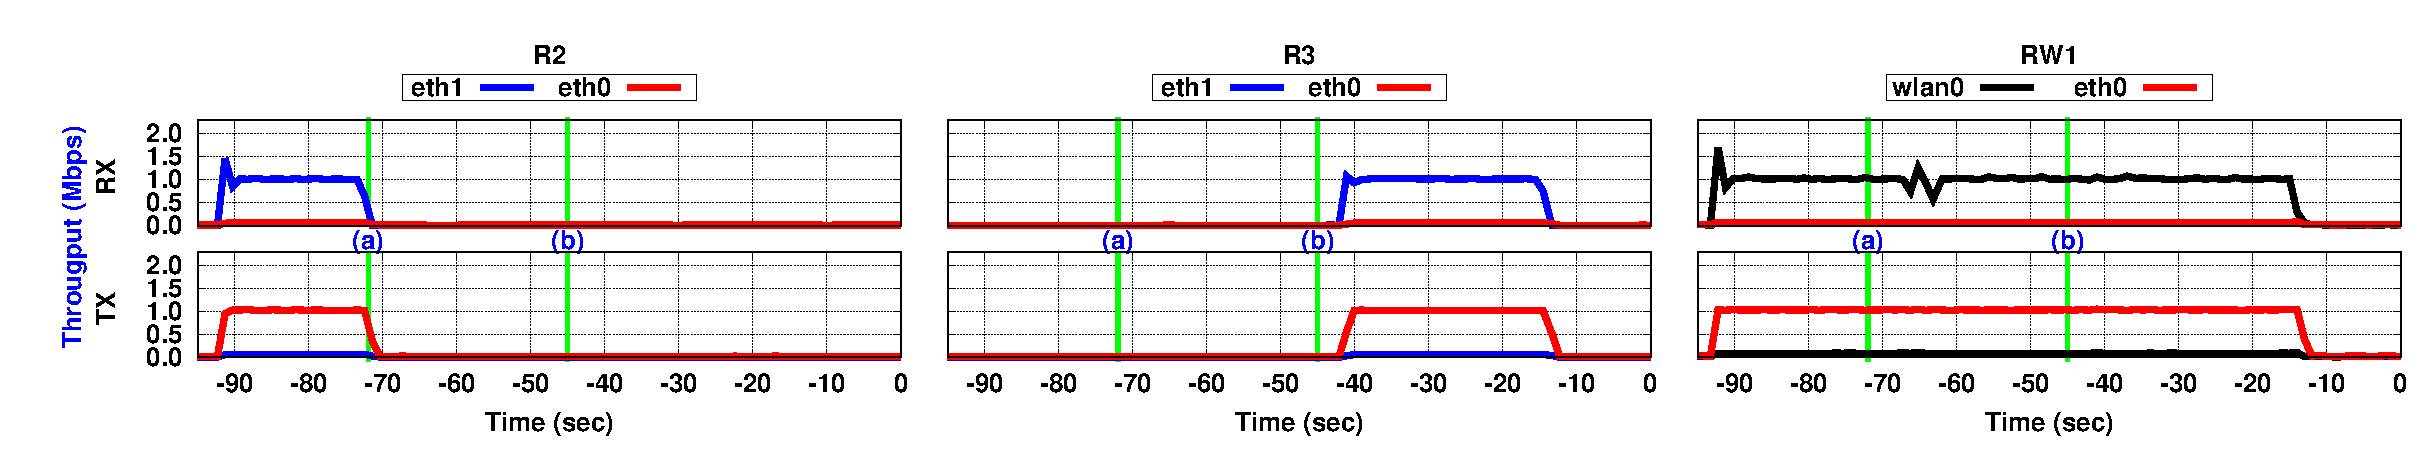
\includegraphics[width=\linewidth]{img/mobility/R2-R3-RW1.eps}
	\caption{\label{fig:mobility_res}RX-TX throughput at different hosts and routers}
\end{figure*}

In Fig.~\ref{fig:rocketfuel_goodput} and Fig.~\ref{fig:rocketfuel_time}, we have shown few selected results. There are two observation we can get from these plot. Firstly, In all of the cases, Viscous performs as good as the MPQUIC. In fact, the Viscous out performed the MPQUIC in reverse flow experiment. It is because Viscous is true multi-path-multi-stream protocol, while the QUIC is not a multi-path protocol. The MPTCP is not as multi-stream protocol, so it required new connection for each transmission. The MPQUIC is multi-path multi-stream protocol, but it suffers for reverse flow because, it can not take advantage of multiple interface during sending a datagram due the UDP api limitation. Viscous does not suffers in the reverse flow experiments because the Viscous use Packet-Socket api.


\subsection{Experiment on mobility}
We perform an experiment on mobility. To test this feature, we prepare the test platform using Raspberry Pi 3. We have depicted the setup diagram in Fig.~\ref{fig:mobility_diagram}. There are total five Raspberry pi acting as routers, this are R1, R2, R3, R4 and RW1. Two host T1 and T2 with this setup. The T1 host directly connected to R1. The host T2 connected to RW1 using WiFi channel. The T2 host is also connected to R3, R4 router via wire. The host T2 can stay connected with R4 or R3 at a time, not with both. All the links except link between RW1 and T2 in this setup are wired link.

To performs the experiment, we start sending data from T2 to T1 while T2 is connected with R4 via wired link and RW1 via WiFi. While the Viscous connection is live, we disconnect T2 from R4. After few seconds, we connect T2 with R3. 

We have shown the result in Fig.~\ref{fig:mobility_res}. In these plots, we have depicted in-coming (RX) and out-going (TX) throughput for each network interfaces for two hosts and 4 routers two covers all the paths between T1 and T2. Top plots depict RX throughput over time and bottom plot depict TX throughput over time for each hosts and routers. Now, we disconnect the link between R4 and T2 at -65th seconds (marked as {\tt a} in plots) and we connect T2 with R3 at time -55 seconds (marked as {\tt b} in plots).

We can see that the Viscous handles mobility pretty. It easily detect the closed link and turn off data transmission through that link. It can also detect new link and establish a channel through new link. We can see it takes few seconds to establish a new connection. It is happening because we are using external tool NetworkManager to provided network connection-disconnection event to the Viscous for now.


\section{Experimental Setup}
\label{exp}

To evaluate the performance of Viscous, we compare the Viscous with popular transport protocols MPTCP, MPQUIC\cite{mpquic-measure}, TCP and QUIC with different network configurations. We performs three different experiments, a) general evaluation with rocket fuel topology, b) aggregated benefit measurement and c) mobility analysis. The Mininet platform is used to perform experiments on rocket fuel topology and aggregated benefit measurement and Raspberry pi board is used to perform experiments on mobility analysis. 

The mininet provides capability of generating different type of network topology with different network conditions in a single system and run any existing real network application on the Mininet generated network. Raspberry pi board setup give us capability to create physical network and run applications on low end devices.

For the Mininet based experiments, we use a computer with 8GB RAM, 4 core GenuineIntel i5-4590 CPU with 3.30 GHz clock frequency. It is equipped with Ubuntu 16.04.1 operating system with Linux kernel version 4.4.70 with the MPTCP v0.92 and the Mininet 2.2.2. For the Rapsberry pi setup, we use Raspberry Pi model 3.
To compare with the QUIC and the MP-QUIC, we use golang implementation of the MP-QUIC by Conick {\it et. al.}~\cite{mpquic-measure} which is a extension of \texttt{golang} implementation of the QUIC~\cite{quic-go}.

\subsection{Setup for General Evaluation with Rocketfuel Topology}
\label{expsetup-rocketfuel}
The RocketFuel topology is a standard topology generated by using {\tt traceroute} from different locations all over the globe to different servers \cite{Spring:2004:MIT:973492.973494}. We take a topology with 29 different networks connected via 15 routers. We place 14 host inside different networks. Among these 14 hosts, we connect 7 hosts with two different networks (we call it client host) and other 7 hosts with a single network (server host). So, there are 7 pair of server-client host. In this topology we use 3 different bandwidth for different links i.e. core link, server link, and client link. A core links connects a switch with a router with 100mbps bandwidth and 3ms delay, a server link connects a server and a switch with 50mbps bandwidth and 2ms delay. We keep 10mbps bandwidth for client link connecting a client host and a switch while varying the delay over different experiment.

In experiments, we sent data from each server host to their dedicated client host using different protocols (Viscous, QUIC, MPQUIC, TCP and MPTCP) and other way around. We call forward experiment when we send traffic from server host to client host and reverse experiment when we send data from client host to server host.

In this experiment, we vary client link delay and number of simultaneous thread. Then we send $50$\footnote{Golang implementation of QUIC and MP-QUIC does not support more than $50$ connections.} back-to-back connection through each thread with payload varied using exponential distribution with mean $25$ KB\footnote{We decided $25$ KB as our initial observation with multiple rich webpages (web page with lots of images and embedding) yields mean HTTP response size of $~25$ KB.}. 

\subsection{Setup for Aggregated Benefit Measurement}
To compare Viscous with other protocol in various network conditions, we perform similar experiment performed by \cite{mpquic-measure,Paasch:mptcp:compare}. We perform these experiments with various of scenarios by changing basic network parameters {\it e.g.} link bandwidth, RTT, queuing delay and packet loss rate. These experiments are performed using simple topology shown in Fig.~\ref{fig:aggregation_dia} with the help of Mininet network emulator. We run experiments on approximately 150 scenarios generated using WSP space filling algorithm described in \cite{wspalgo} from configuration space described in Table~\ref{tbl:noloss_param}. Three experiments are performed on each scenario for each protocol. We run experiments on TCP and QUIC for both the paths and compared with best performance. We also observed that the MPTCP depends on initial path selection, so we run experiments with MPTCP for both the paths and compared with best and worst initial path performance. We considered Goodput as the metric of performance. In each of these experiments, we send 50 back-to-back request-response over a single thread. The client request for a payload size (in number of bytes) to server and the server transfer the requested amount of payload to client. We vary response size with a exponential distribution with mean $25$ KB payload.
\begin{equation} \label{eqn:agre_benefit}
Ben(S) = 
\begin{cases}
\frac{G_v - G_p^{max}}{G_v - G_v^{max}} & \text{if } G_v > G_V^{max} \\
\frac{G_v - G_p^{max}}{G_v^{max}} & \text{otherwise}
\end{cases}
\end{equation}

To measure aggregative benefit, we followed modified equation provided in \cite{Kaspar:2012:MAH:2206765.2206770,Paasch:mptcp:compare,mpquic-measure}
as Equation~(\ref{eqn:agre_benefit}). Here we measure the benefit of using Viscous instead of other protocol for a given scenario $S$. Here $G_v$ is the mean Goodput found in all experiments using Viscous for the scenario $S$, $G_p^{max}$ is the max of mean Goodput found in each path for single path protocol while $G_p^{max}$ is mean Goodput achieved by a multi-path protocol. The value of $Ben(S)$ is in between -1 to 1, while -1 mean Goodput of other protocol is twice good as Viscous while 1 mean, Goodput of other protocol is 0, and if $Ben(S)$ is 0, other protocol perform exactly same as Viscous.

\begin{figure}
	\centering
	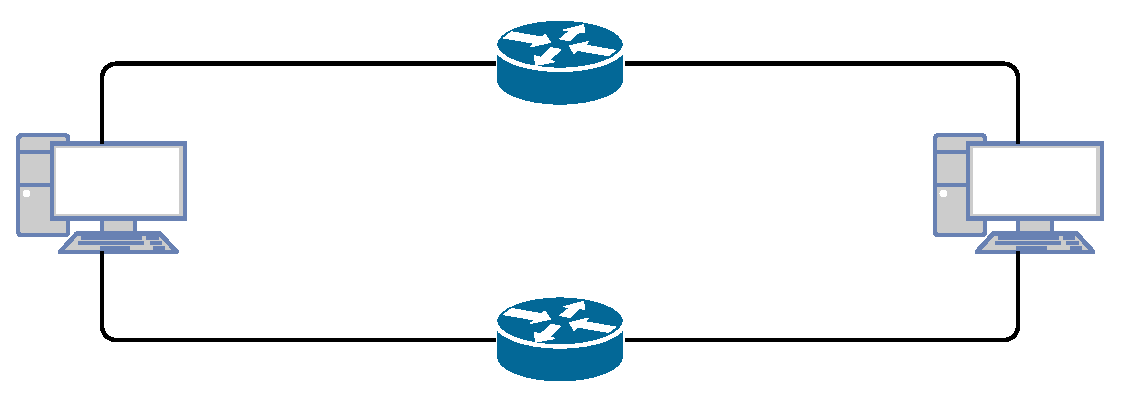
\includegraphics[width=\linewidth]{img/aggregation.eps}
	\caption{\label{fig:aggregation_dia}Network used to find aggregative benefit}
\end{figure}

\begin{table}[h]
	\centering
	\begin{tabular}{l||c|c||c|c}
		%		\hline
		& \multicolumn{2}{c||}{Low-BDP} & \multicolumn{2}{c}{High-BDP}\\
		\hline
		\hline
		Capacity [Mbps] & 0.1 & 100 & 0.1 & 100 \\
		\hline
		Propagation delay [ms] & 0 & 50 & 0 & 400 \\
		\hline
		Queuing [ms] & 0 & 100 & 0 & 2000 \\
		\hline
		Loss rate [\%] & 0 & 2.5 & 0 & 2.5 \\
		%		\hline
	\end{tabular}
	\caption{\label{tbl:noloss_param}Scenario used}
\end{table}

\subsection{Setup for Mobility Analysis}
We perform an experiment on mobility. To test this feature, we prepare the test platform using Raspberry Pi 3. We have depicted the setup diagram in Fig.~\ref{fig:mobility_diagram}. There are total five Raspberry pi acting as routers, this are R1, R2, R3, R4 and RW1. Two host T1 and T2 with this setup. The T1 host directly connected to R1. The host T2 connected to RW1 using WiFi channel. The T2 host is also connected to R3, R4 router via wire. The host T2 can stay connected with R4 or R3 at a time, not with both. All the links except link between RW1 and T2 in this setup are wired link.

To performs the experiment, we start sending data from T2 to T1 while T2 is connected with R4 via wired link and RW1 via WiFi. While the Viscous connection is live, we disconnect T2 from R4. After few seconds, we connect T2 with R3. 
\begin{figure}
	\centering
	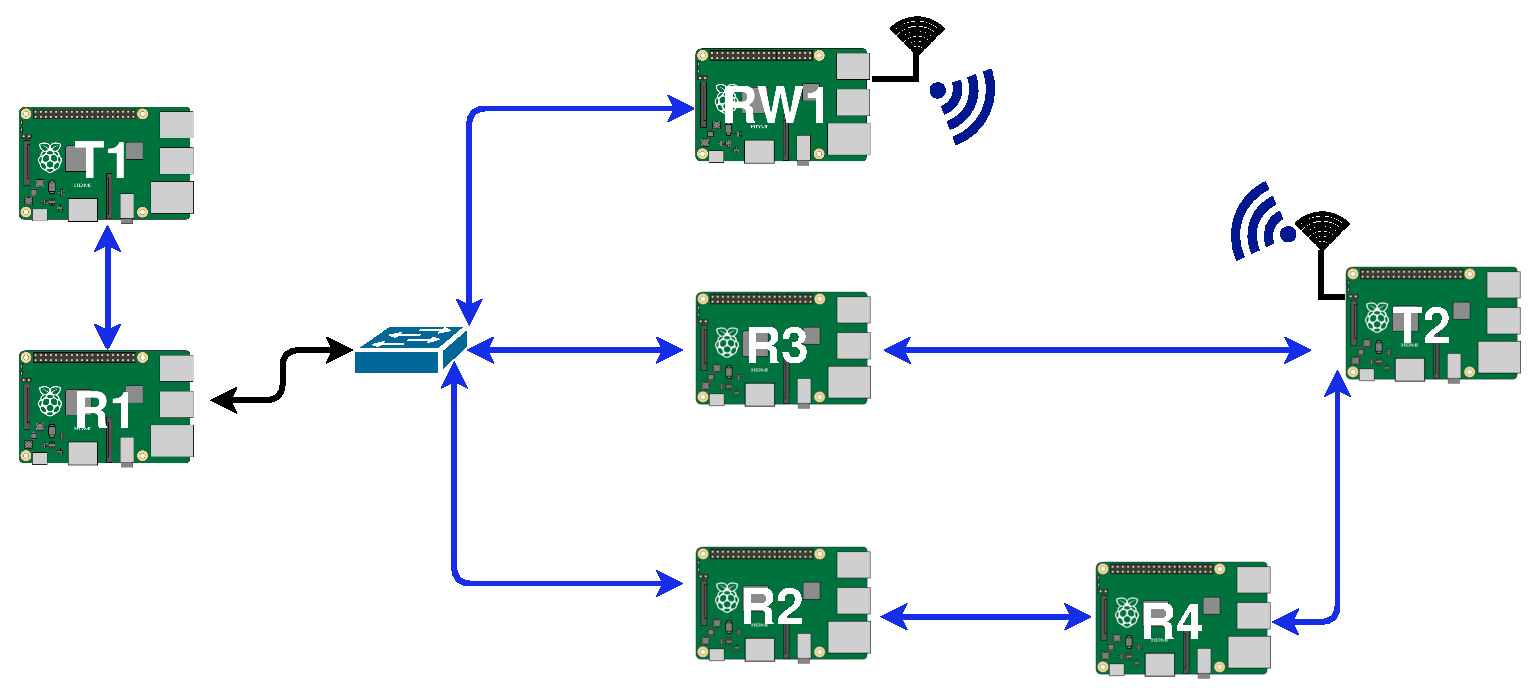
\includegraphics[width=.9\linewidth]{img/mobility/demo-Diagram.eps}
	\caption{\label{fig:mobility_diagram}Raspberry pi setup to test the mobility of viscous}
\end{figure}




\begin{figure*}[h]
%	\captionsetup[subfigure]{}
	\begin{center}
		
		\begin{subfigure}{.49\linewidth}
			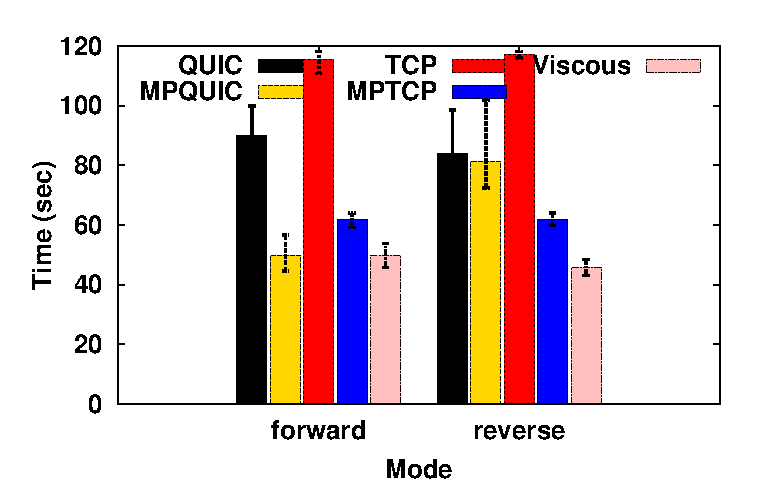
\includegraphics[width=0.95\linewidth]{img/rocketfuel/tymdiff-5-5.eps}
			\caption{\label{fig:rocketfuel_time_5_20}Delay=5ms \#threads=5}
		\end{subfigure}
		\begin{subfigure}{.49\linewidth}
			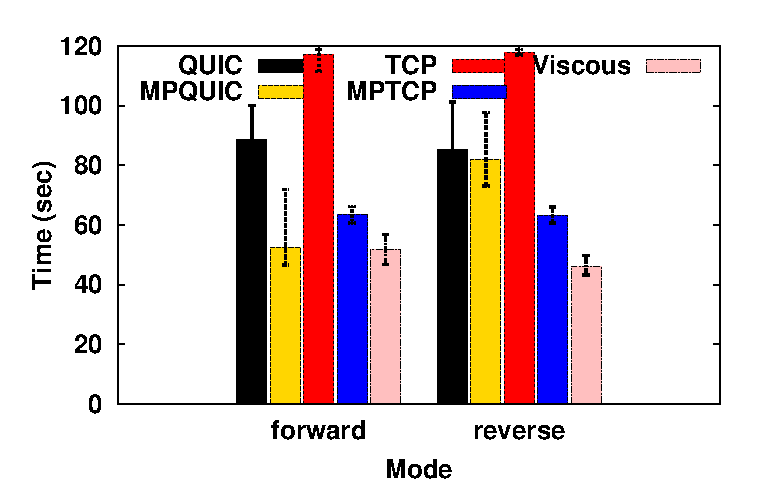
\includegraphics[width=0.95\linewidth]{img/rocketfuel/tymdiff-10-5.eps}
			\caption{\label{fig:rocketfuel_time_10_5}Delay=10ms \#threads=5}
		\end{subfigure}
		\begin{subfigure}{.49\linewidth}
			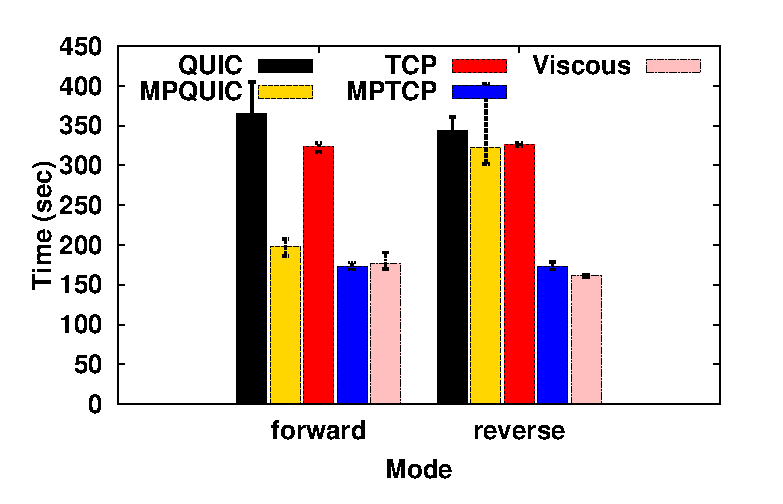
\includegraphics[width=0.95\linewidth]{img/rocketfuel/tymdiff-10-20.eps}
			\caption{\label{fig:rocketfuel_time_10_20}Delay=10ms \#threads=20}
		\end{subfigure}
		\begin{subfigure}{.49\linewidth}
			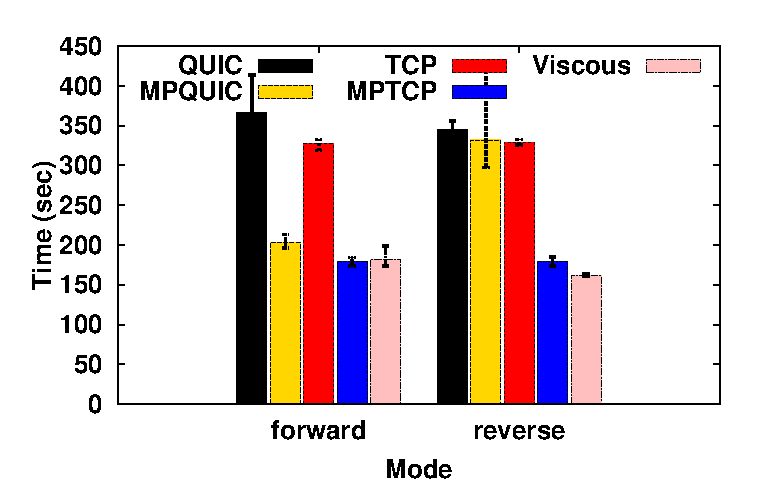
\includegraphics[width=0.95\linewidth]{img/rocketfuel/tymdiff-20-20.eps}
			\caption{\label{fig:rocketfuel_time_20_20}Delay=20ms \#threads=20}
		\end{subfigure}
		\caption{\label{fig:rocketfuel_time}Average average flow completion time over Rocketfuel topology}
	\end{center}
\end{figure*}


\begin{figure*}[h]
	\captionsetup[subfigure]{}
	\begin{center}
		\begin{subfigure}{.49\linewidth}
			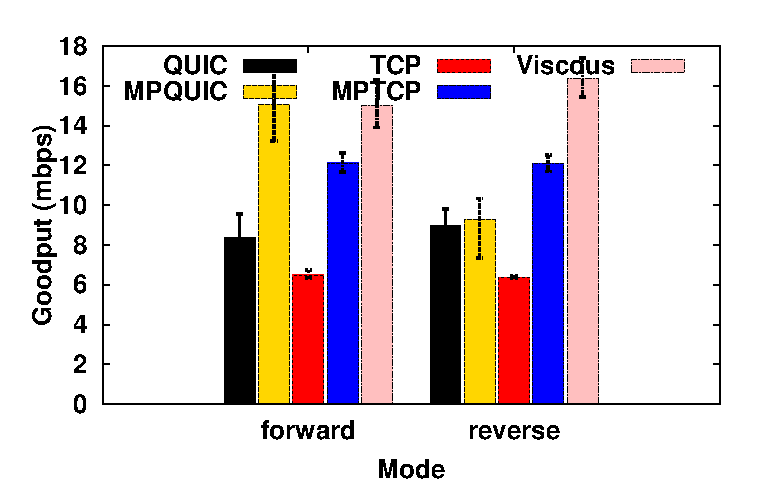
\includegraphics[width=0.95\linewidth]{img/rocketfuel/goodPut-5-5.eps}
		 \caption{\label{fig:rocketfuel_goodput_5_20}Delay=5ms \#threads=5}
		\end{subfigure}
		\begin{subfigure}{.49\linewidth}
			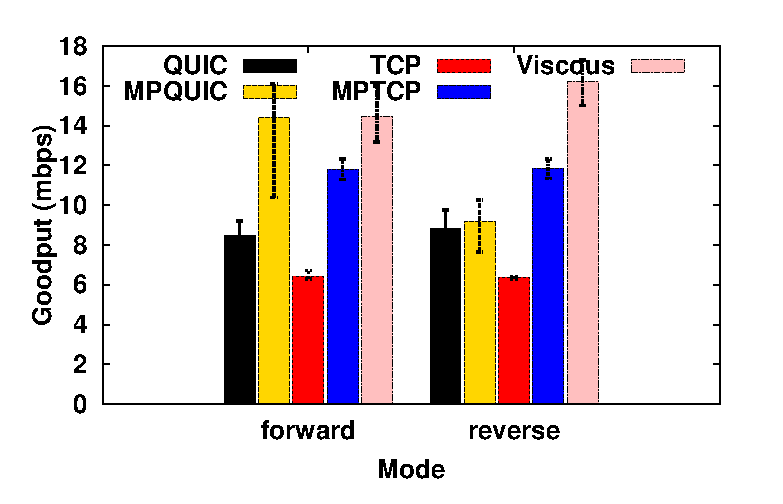
\includegraphics[width=0.95\linewidth]{img/rocketfuel/goodPut-10-5.eps}
		 \caption{\label{fig:rocketfuel_goodput_10_5}Delay=10ms \#threads=5}
		\end{subfigure}
		\begin{subfigure}{.49\linewidth}
			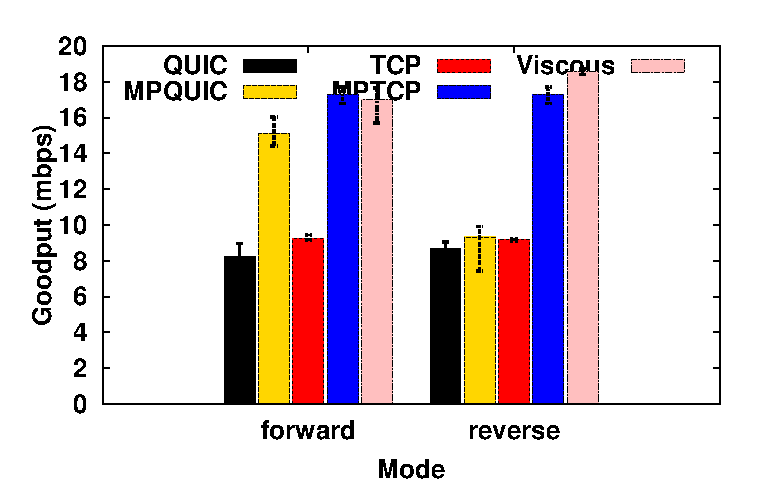
\includegraphics[width=0.95\linewidth]{img/rocketfuel/goodPut-10-20.eps}
		 \caption{\label{fig:rocketfuel_goodput_10_20}Delay=10ms \#threads=20}
		\end{subfigure}
		\begin{subfigure}{.49\linewidth}
			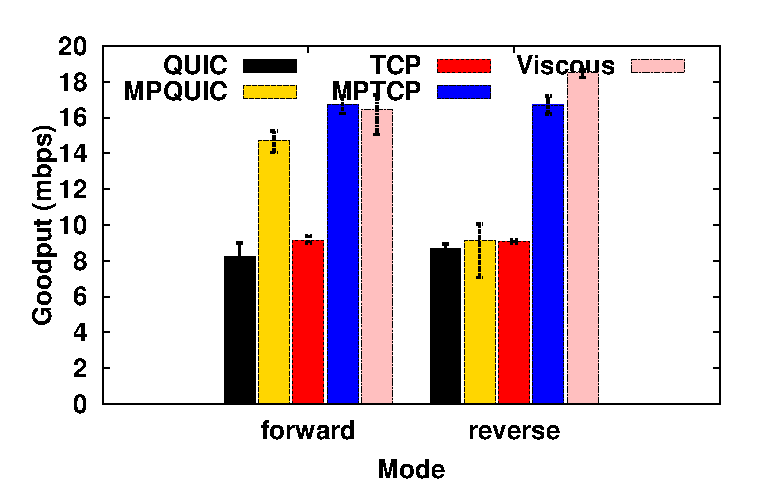
\includegraphics[width=0.95\linewidth]{img/rocketfuel/goodPut-20-20.eps}
		 \caption{\label{fig:rocketfuel_goodput_20_20}Delay=20ms \#threads=20}
		\end{subfigure}
		\caption{\label{fig:rocketfuel_goodput}Average GoodPut over Rocketfuel topology}
	\end{center}
\end{figure*}
\section{Results}
Previous section we have describe the different experimental setup. In this section, we analyze the results of those experiments.

\subsection{Overall performance}
We have describe the experimental setup in the section \ref{expsetup-rocketfuel}.
In Fig.~\ref{fig:rocketfuel_time} and Fig.~\ref{fig:rocketfuel_goodput}, we have shown few selected results. There are two observation we can get from these plot. Firstly, in all of the cases, Viscous performs as good as the MPQUIC. In fact, Viscous out performed MPQUIC in reverse flow experiment. It is happening because Viscous is true multi-path-multi-stream protocol, while QUIC is not a multi-path protocol. MPTCP is not a multi-stream protocol, so it required new connection for each transmission. MPQUIC is multi-path multi-stream protocol, but it suffers for reverse flow because, it can not take advantage of multiple interface during sending a datagram due the UDP api limitation. Viscous does not suffers in the reverse flow experiments because the Viscous use Packet-Socket api.



\subsection{Aggregated Benefit Measurement}

\begin{figure}
	\captionsetup[subfigure]{}
	\begin{center}
		\begin{subfigure}{.49\linewidth}
			\includegraphics[width=.95\linewidth]{img/lowbdp-lossless/lowbdpnoloss_benefit.eps}
		 \caption{\label{fig:benefit-box} Benefit of Viscous over other transport different protocol}
		\end{subfigure}
		\begin{subfigure}{.49\linewidth}
			\includegraphics[width=.95\linewidth]{img/lowbdp-lossless/lowbdpnoloss_cdf.eps}				 
		 \caption{\label{fig:benefit-cdf} CDF of benefit of Viscous over other transport different protocol}
		\end{subfigure}
		\caption{\label{fig:benefit}Experimental results on lossless low BDP channels}
	\end{center}
\end{figure}

In Fig.~\ref{fig:benefit}, \ref{fig:benefit-high}, \ref{fig:benefit-lossy} and \ref{fig:benefit-high-lossy}, we have depicted the result of our experiment on aggregated benefit of Viscous.
We can see that the Viscous is performing better than all the other protocols in all the scenarios. It can be understood that, the TCP and the MPTCP aren't performing good enough because they need to go through slow-start phase for every request. A loss of a packet during slow start state can reduce throughput of TCP and MPTCP greatly as it causes unsaturated reduction of the $cwnd$. However QUIC and MP-QUIC should not have such problem as they uses multiple types of signal to understand congestion. So, after taking close look to we found that QUIC and MP-QUIC have strict flow control mechanism at connection level to by setting receivers' window size to 3.5MB. This flow control causing the reduction of the speed for the QUIC and MP-QUIC while the Bandwidth or the RTT of the link is little higher (i.e. BDP is higher that $3.5$ MB). However, Viscous do not have such connection level flow control. It have flow control only at the flow layer. So, Viscous is performing better even in case of lossy channel.

\begin{figure}
	\captionsetup[subfigure]{}
	\begin{center}
		\begin{subfigure}{.49\linewidth}
			\includegraphics[width=.95\linewidth]{img/highbdp-lossless/highbdpnoloss_benefit.eps}
		 \caption{\label{fig:benefit-box-high} Benefit of Viscous over other transport different protocol}
		\end{subfigure}
		\begin{subfigure}{.49\linewidth}
			\includegraphics[width=.95\linewidth]{img/highbdp-lossless/highbdpnoloss_cdf.eps}
		 \caption{\label{fig:benefit-cdf-high} CDF of benefit of Viscous over other transport different protocol}
		\end{subfigure}
		\caption{\label{fig:benefit-high}Experimental results on lossless high BDP channels}
	\end{center}
\end{figure}


\begin{figure}
	\captionsetup[subfigure]{}
	\begin{center}
		\begin{subfigure}{.49\linewidth}
			\includegraphics[width=.95\linewidth]{img/lowbdp-lossy/lowbdplossy_benefit.eps}
		 \caption{\label{fig:benefit-box-lossy} Benefit of Viscous over other transport different protocol}
		\end{subfigure}
		\begin{subfigure}{.49\linewidth}
			\includegraphics[width=.95\linewidth]{img/lowbdp-lossy/lowbdplossy_cdf.eps}
		 \caption{\label{fig:benefit-cdf-lossy} CDF of benefit of Viscous over other transport different protocol}
		\end{subfigure}
		\caption{\label{fig:benefit-lossy}Experimental results on lossy low BDP channels}
	\end{center}
\end{figure}

\begin{figure}
	\captionsetup[subfigure]{}
	\begin{center}
		\begin{subfigure}{.49\linewidth}
			\includegraphics[width=.95\linewidth]{img/highbdp-lossy/highbdplossy_benefit.eps}
		 \caption{\label{fig:benefit-box-high-lossy} Benefit of Viscous over other transport different protocol}
		\end{subfigure}
		\begin{subfigure}{.49\linewidth}
			\includegraphics[width=.95\linewidth]{img/highbdp-lossy/highbdplossy_cdf.eps}
		 \caption{\label{fig:benefit-cdf-high-lossy} CDF of benefit of Viscous over other transport different protocol}
		\end{subfigure}
		\caption{\label{fig:benefit-high-lossy}Experimental results on lossy high BDP channels}
	\end{center}
\end{figure}


\begin{figure*}[h]
	\centering
	\includegraphics[width=\linewidth]{img/mobility/T1-T2-R1.eps}
	\includegraphics[width=\linewidth]{img/mobility/R2-R3-RW1.eps}
	\caption{\label{fig:mobility_res}RX-TX throughput at different hosts and routers}
\end{figure*}


\subsection{Mobility Support Analysis}

We have shown the result in Fig.~\ref{fig:mobility_res}. In these plots, we have depicted in-coming (RX) and out-going (TX) throughput for each network interfaces for two hosts and 4 routers two covering all the paths between T1 and T2. Top plots depict RX throughput over time and bottom plot depict TX throughput over time for each hosts and routers. Now, we disconnect the link between R4 and T2 at -65th seconds (marked as {\tt a} in plots) and we connect T2 with R3 at time -55 seconds (marked as {\tt b} in plots).

We can see that Viscous handles mobility pretty well. It easily detects the closed link and turn off data transmission through that link. It can also detect new link and establish a channel through the new link. We can see that it takes few seconds to establish a new connection. It is happening because we are using external tool NetworkManager to provided network connection-disconnection event to the Viscous for now.


%\section{Related Work}
Our work is motivated by the network requirement of existing low-end IoT devices and the smart router those are connected to it. 
The concept of multipath is not new. A few efforts have been made to dynamically schedule between multiple interfaces in order to 
improve the network performance, at transport layer as in Multipath \acrshort{tcp} (\acrshort{mptcp}). It provides the power 
to use multiple paths to a regular \acrshort{tcp} session. But as \acrshort{tcp} based on kernel approach and there is need to change 
the \acrshort{tcp} headers, it is not supported by all the available middleboxes. The difference between \acrshort{mpiot} and 
\acrshort{mptcp} is as follows, in case of packet losses, short-time unavailability of a path or fluctuation of on a path \acrshort{mptcp} 
can retransmit packets from one path to another, ideally from slower to faster path. But in the case of \acrshort{mpiot} packets once sent in a path,
will be retransmitted to that path only.


\section{Conclusion}
Considering the limitations of current transmission protocols for today’s diverse device and traffic characteristics, in this report, we have developed Viscous that provides a middleware between the user application and the transport layer to handle end-to-end network characteristics. Viscous is completely compatible with the current network protocol stack, while it provides significant performance boost in the application throughput. It is developed on top of the UDP along with a set of novel features to support mobility, multi-homing and short-lived parallel and sequential flows. From the prototype implementation and performance analysis over an emulated environment, we show that the worst case performance of Viscous is similar to TCP, which indicates its applicability for a wide range of applications. 
In future, our target is to enhance Viscous with application layer QoS support to make it an alternate for both non-real time and real time traffic transport.  Additionally we plan to explore transport of multimedia traffic over multipath protocols. 
\\
\\
\section*{Publications}
[1] Abhijit Mondal, Satadal Sengupta, B.R. Reddy, M.J.V. Koundinya, Chander G., Pradipta De, Niloy Ganguly, Sandip Chakraborty, ``\textit{Candid with YouTube: Adaptive Streaming Behavior and Implications on Data Consumption}'' in Proceedings of the 27th Workshop on Network and Operating Systems Support for Digital Audio and Video (ACM NOSSDAV'17), Taipei, Taiwan, June 20 - 23, 2017 .

[2] Abhijit Mondal, Sourav Bhattacharjee, Sandip Chakraborty, ``\textit{Viscous: An End to End Protocol for Ubiquitous Communication Over Internet of Everything}'' in Proceedings of 42nd Annual IEEE Conference on Local Computer Networks (IEEE LCN 2017), Singapore, October 9-12, 2017.

[3] Abhijit Mondal, Sandip Chakraborty, ``\textit{An End-to-end protocol over Heterogeneous Internet}'', \textbf{submitted} to IEEE/ACM Transaction on Networking.
\\
\\

%


% use section* for acknowledgment
\ifCLASSOPTIONcompsoc
  % The Computer Society usually uses the plural form
  \section*{Acknowledgments}
\else
  % regular IEEE prefers the singular form
  \section*{Acknowledgment}
\fi


The authors would like to thank...






\bibliographystyle{IEEEtranS}
\bibliography{ref/lcnref.bib,ref/rfcref.bib} 
\end{document}


